\chapter{Invariant mass fits to $\Bd\to\Kstarz\ll$ simulated candidates}
\phantomsection\label{app:RKMCfits}

This appendix contains fits to the $m(K\pi \mu\mu)$ and $m(K\pi ee )$ invariant mass of $\Bd\to\Kstarz\ll$ simulated candidates
used to constrain parameters in the fit to data.

\begin{figure}[h!]
\centering
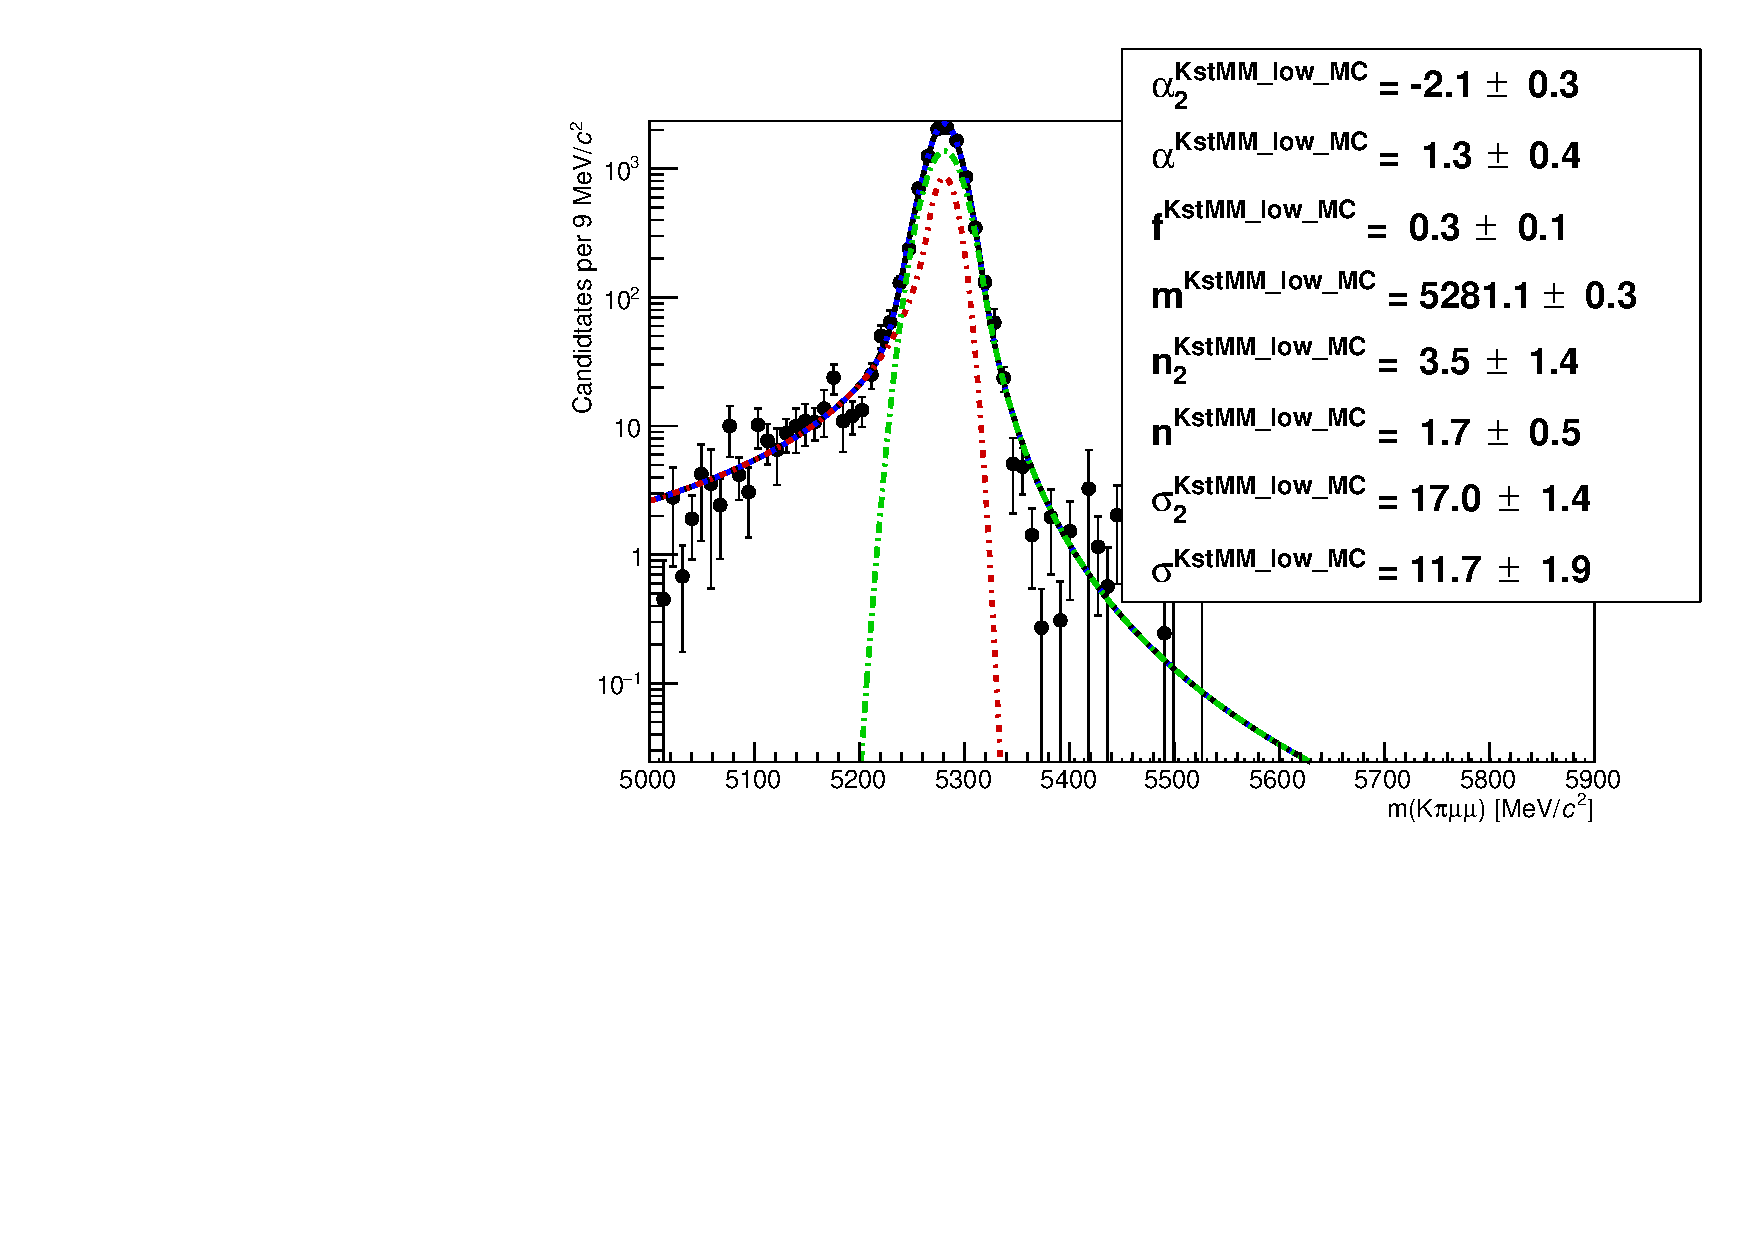
\includegraphics[width=0.55\textwidth]{RKst/figs/Fit/fit_MM/KstMM_low_MC_log.pdf} \\
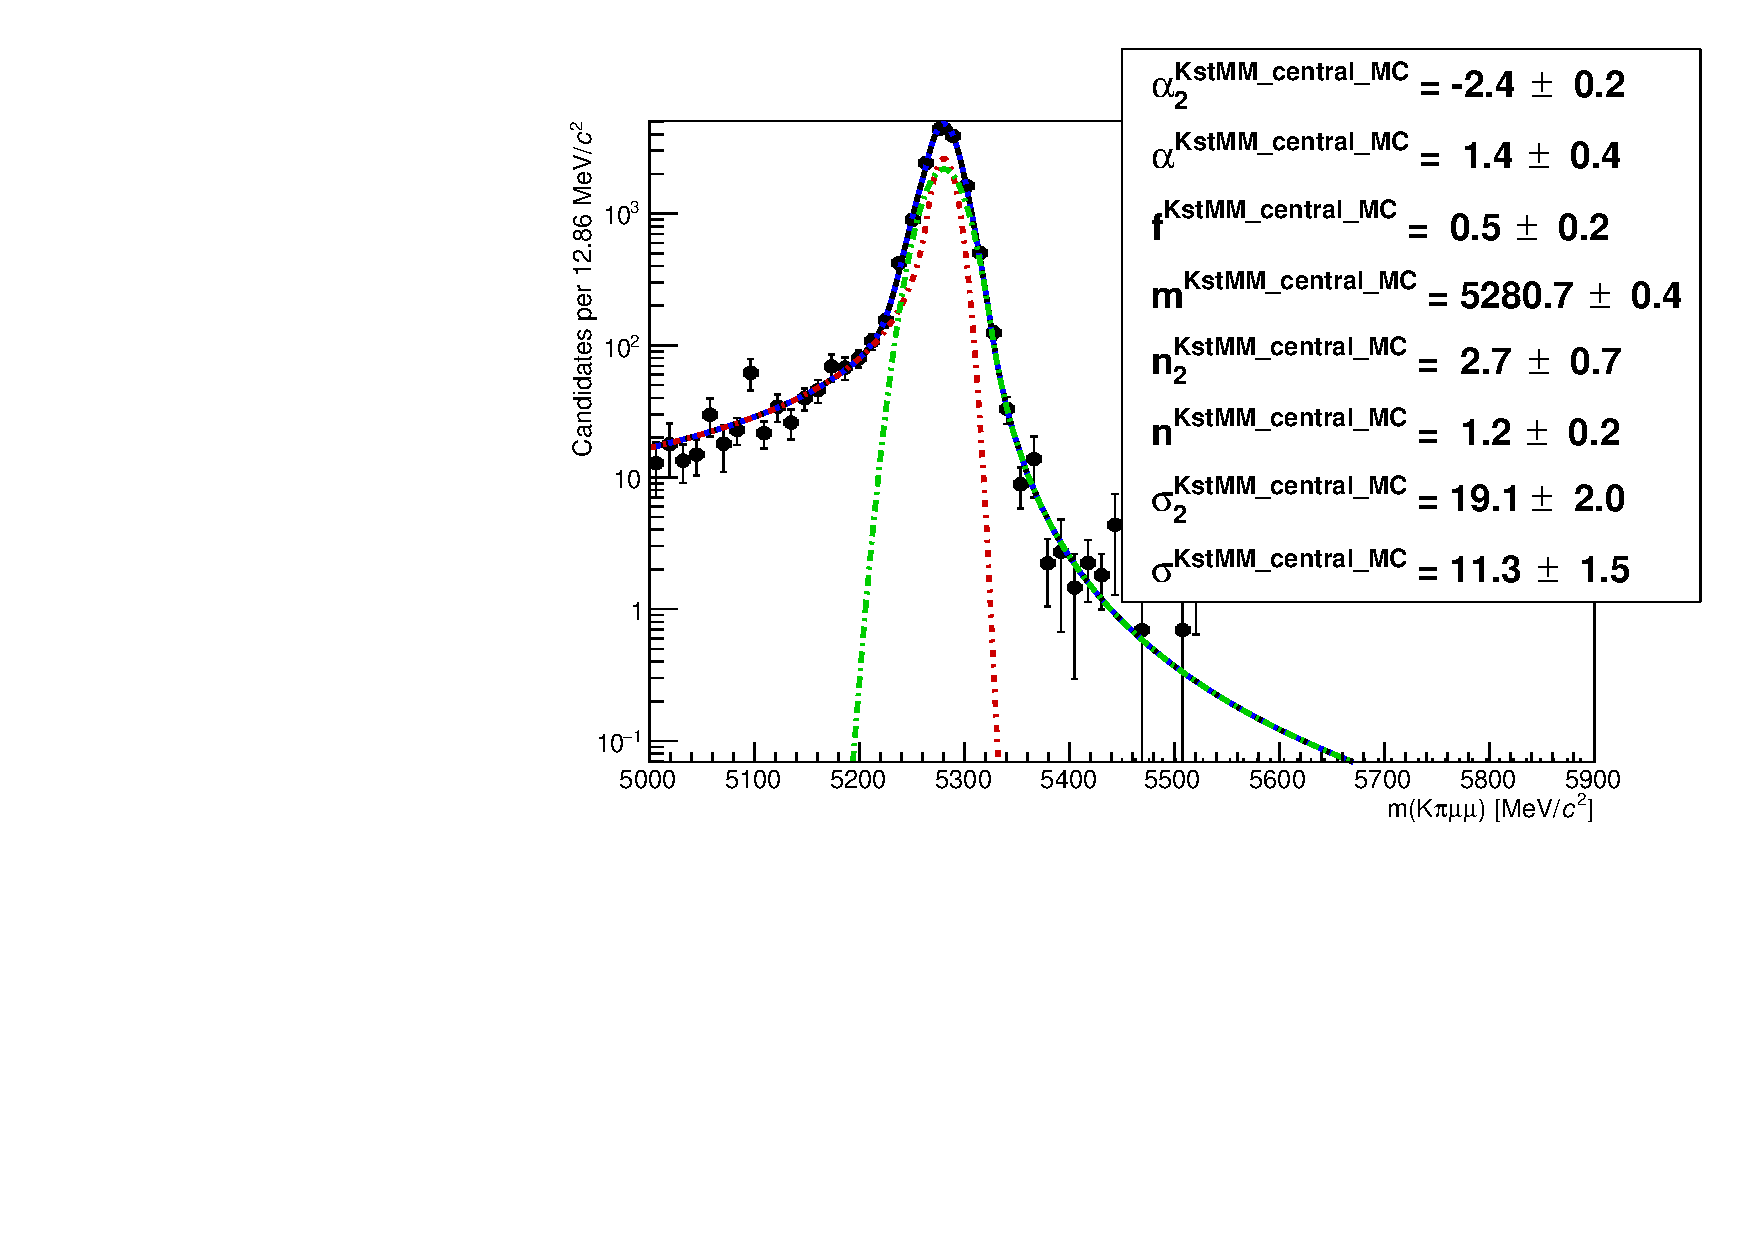
\includegraphics[width=0.55\textwidth]{RKst/figs/Fit/fit_MM/KstMM_central_MC_log.pdf} \\
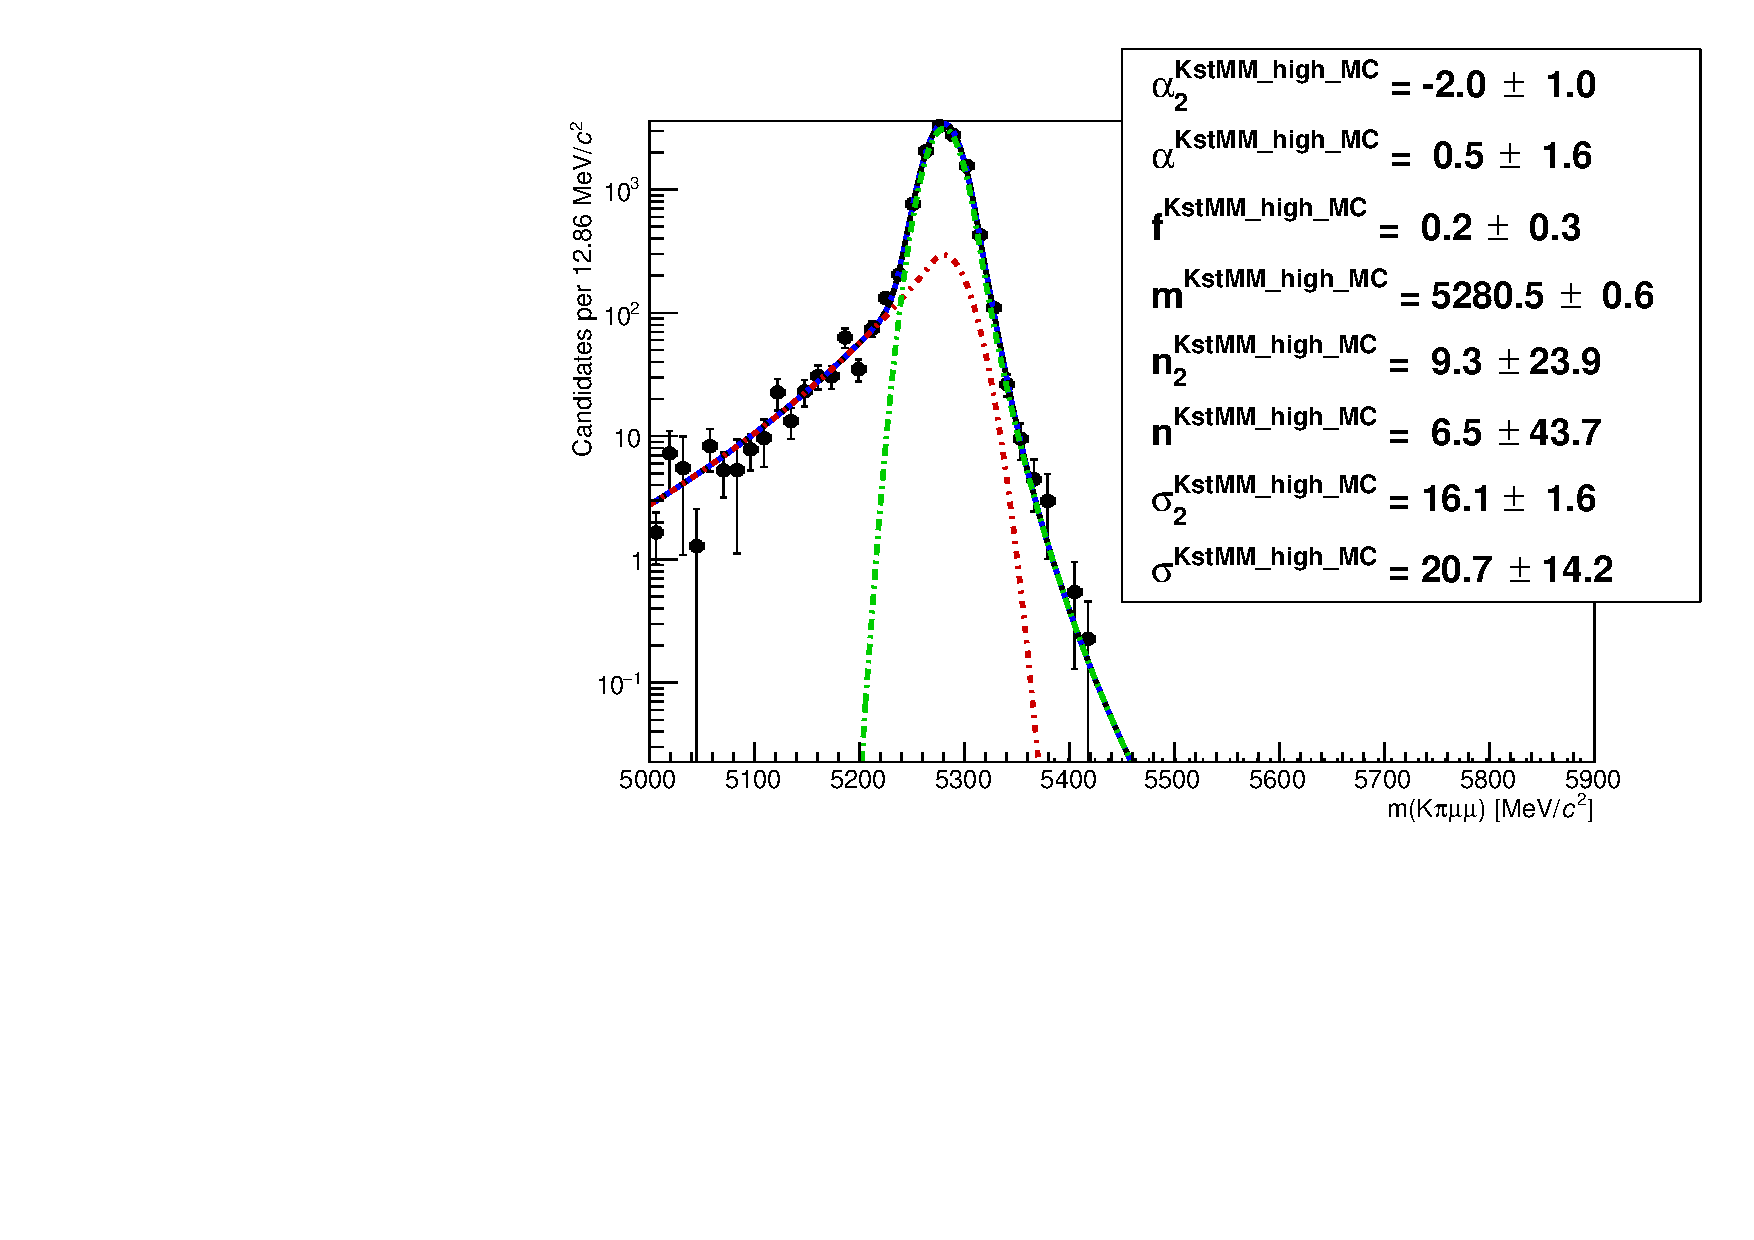
\includegraphics[width=0.55\textwidth]{RKst/figs/Fit/fit_MM/KstMM_high_MC_log.pdf}
\caption{Fitted $m(K\pi \mu\mu)$ mass spectrum for simulated events in the
low (top), central (medium) and high (bottom) \qsq intervals. }
\label{fig:mumu_MC_fits}
\end{figure}

\begin{figure}[h!]
\centering
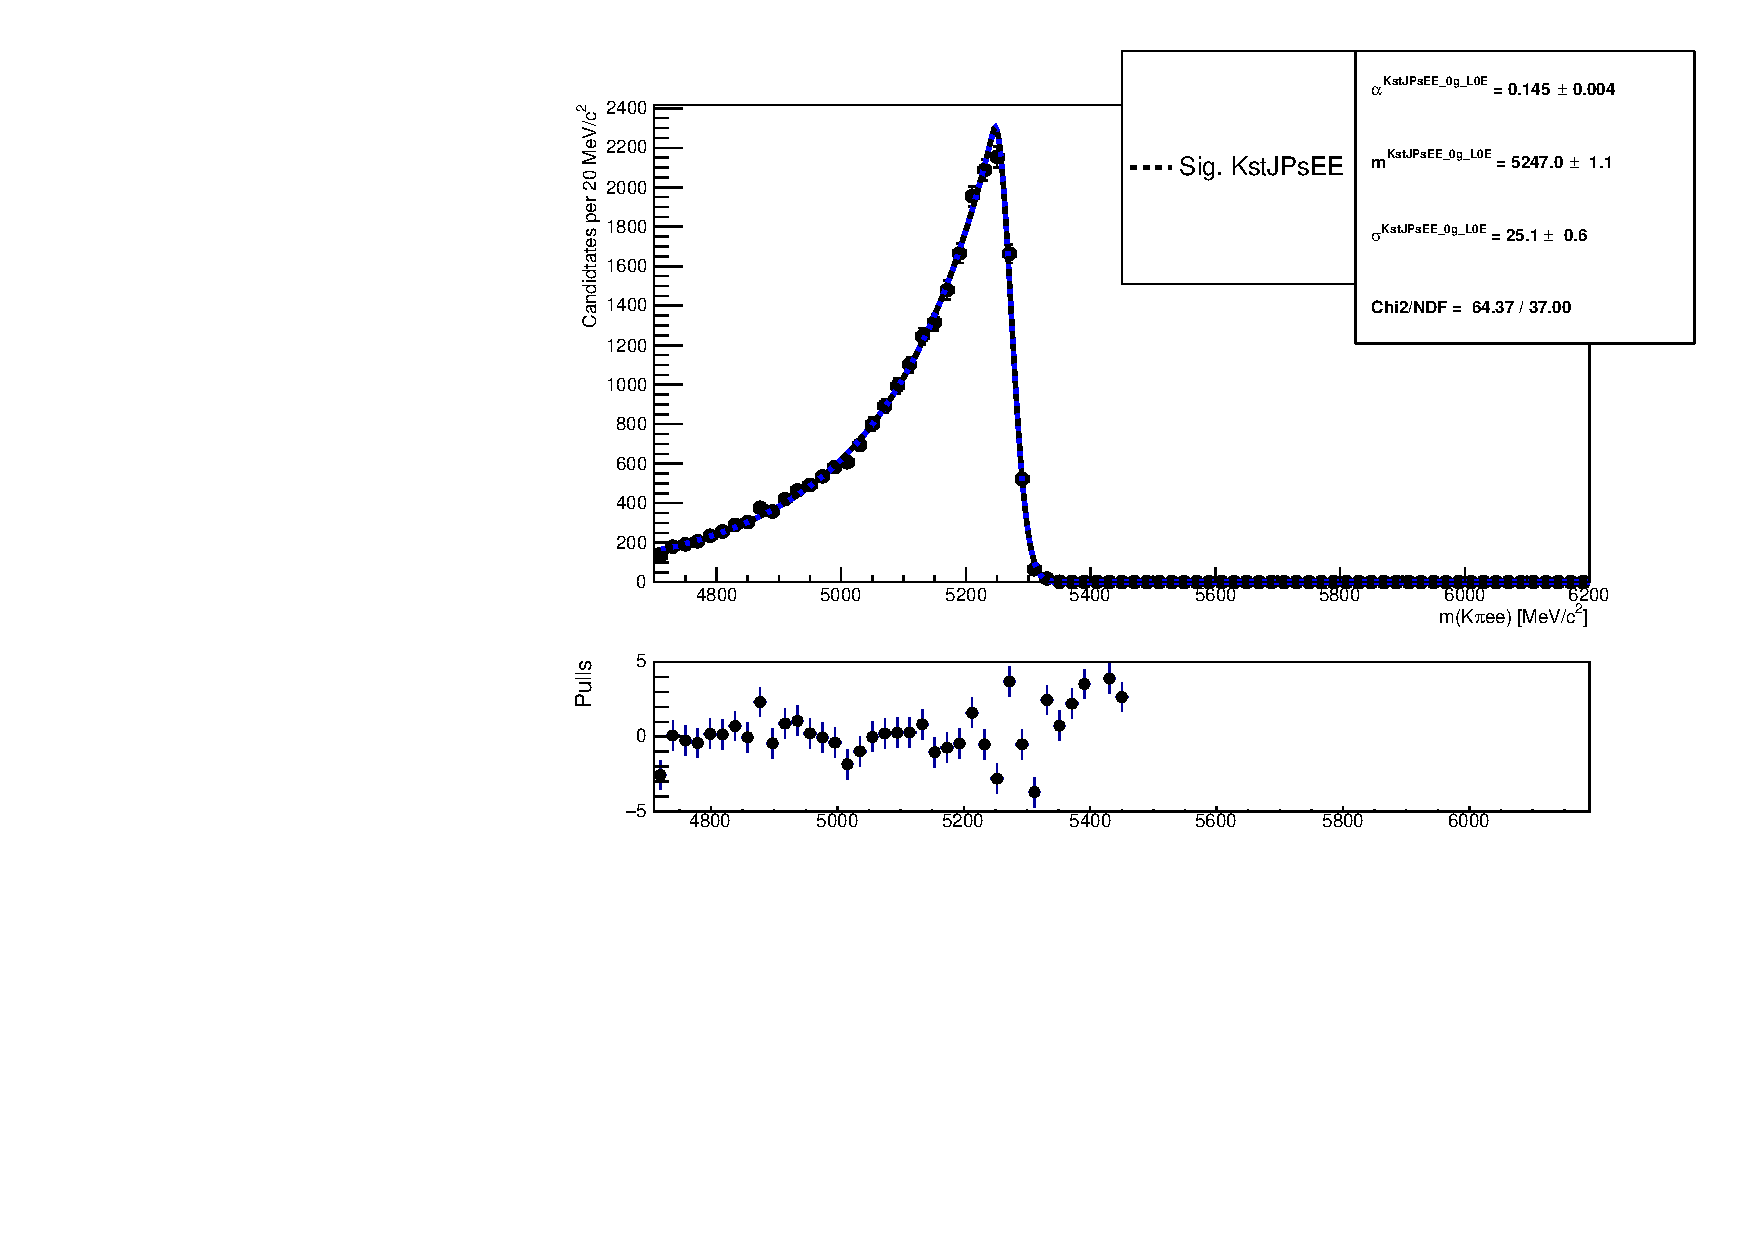
\includegraphics[width=0.6\textwidth]{RKst/figs/fit_EEs_0_EE-q2central-gmc/KstJPsEE_0g_L0E_fitAndRes.pdf}
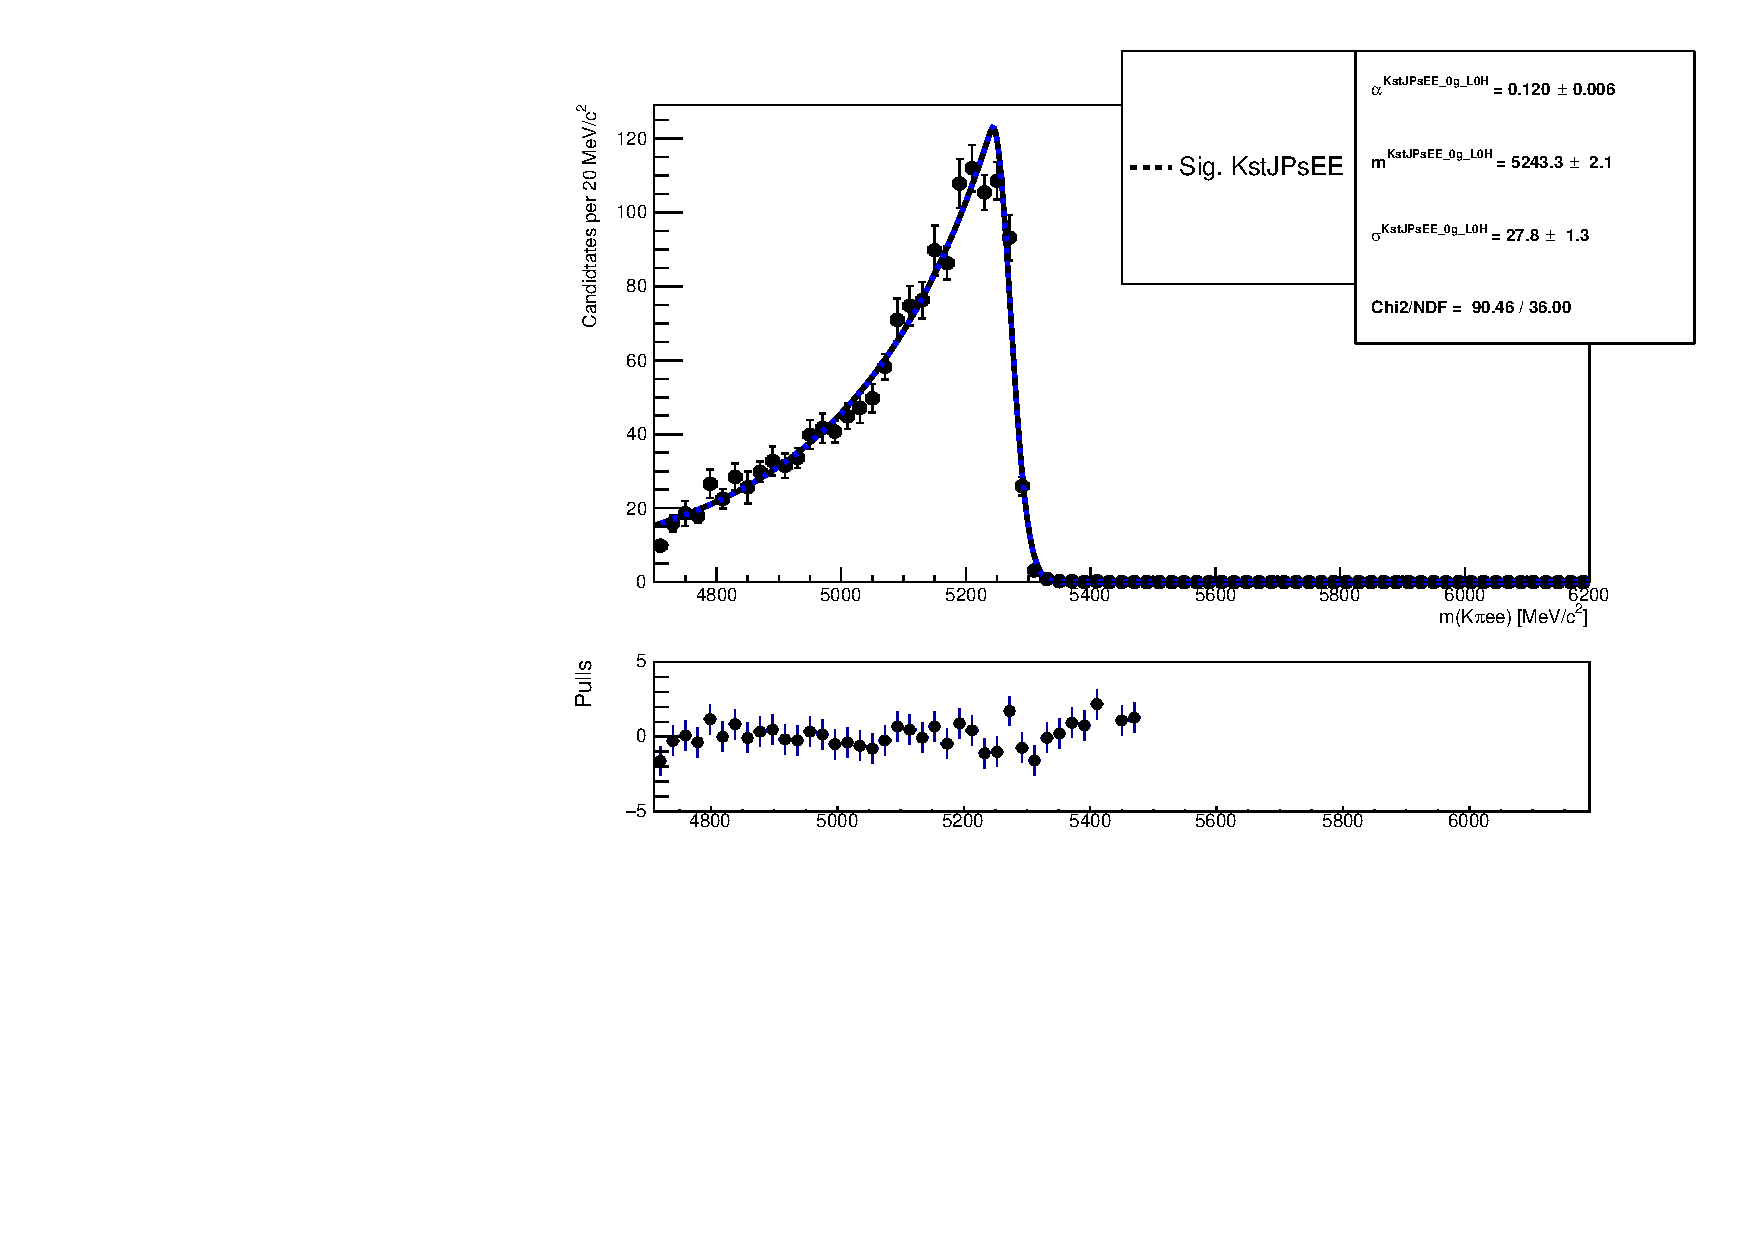
\includegraphics[width=0.6\textwidth]{RKst/figs/fit_EEs_0_EE-q2central-gmc/KstJPsEE_0g_L0H_fitAndRes.pdf}
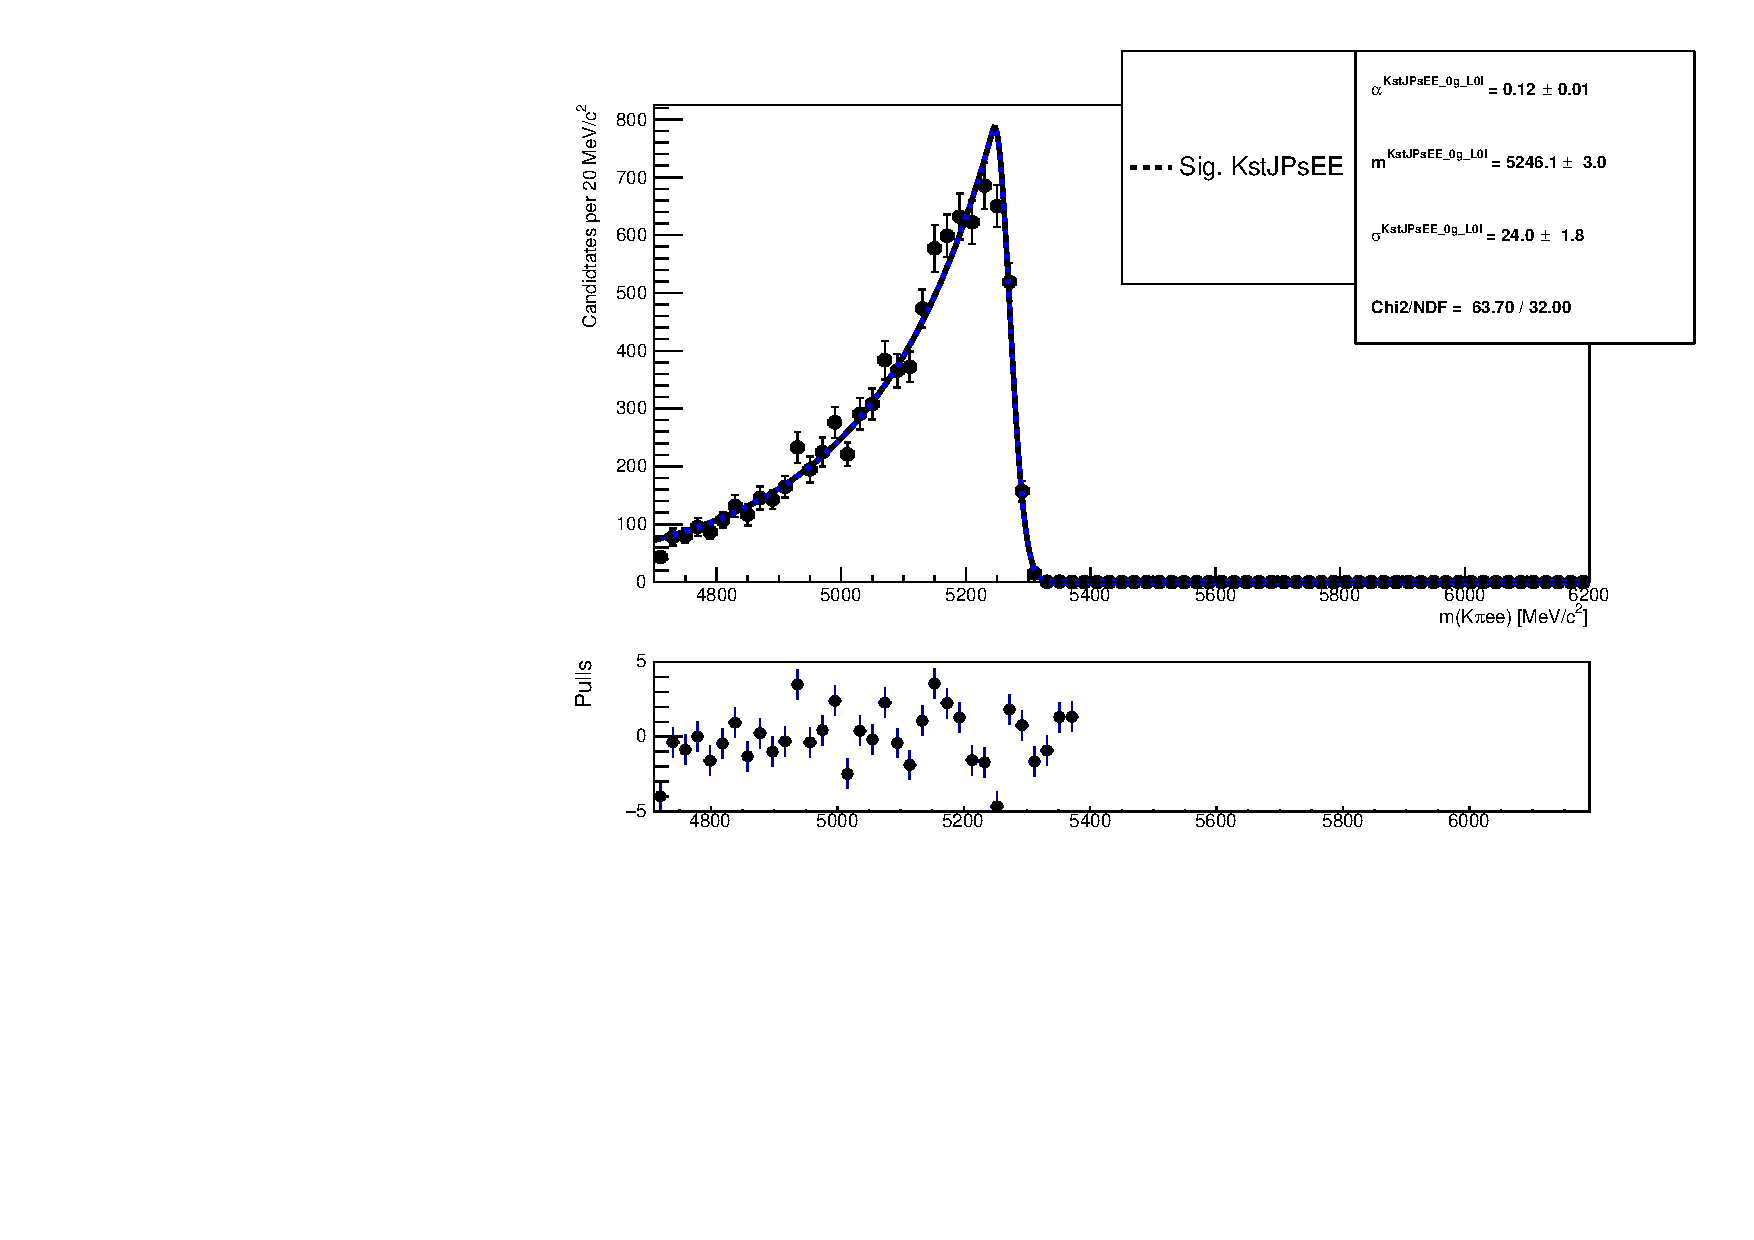
\includegraphics[width=0.6\textwidth]{RKst/figs/fit_EEs_0_EE-q2central-gmc/KstJPsEE_0g_L0I_fitAndRes.pdf}
\caption{Fitted $m(K\pi ee)$ mass spectrum of $B^0 \rightarrow K^{*0} J/\psi(J/\psi\rightarrow ee)$ simulated
events in the three trigger categories and no photon emitted. }
\label{fig:FitEE_MC_inTrigCat_Brem0}
\end{figure}
%
%\clearpage
\begin{figure}[h!]
\centering
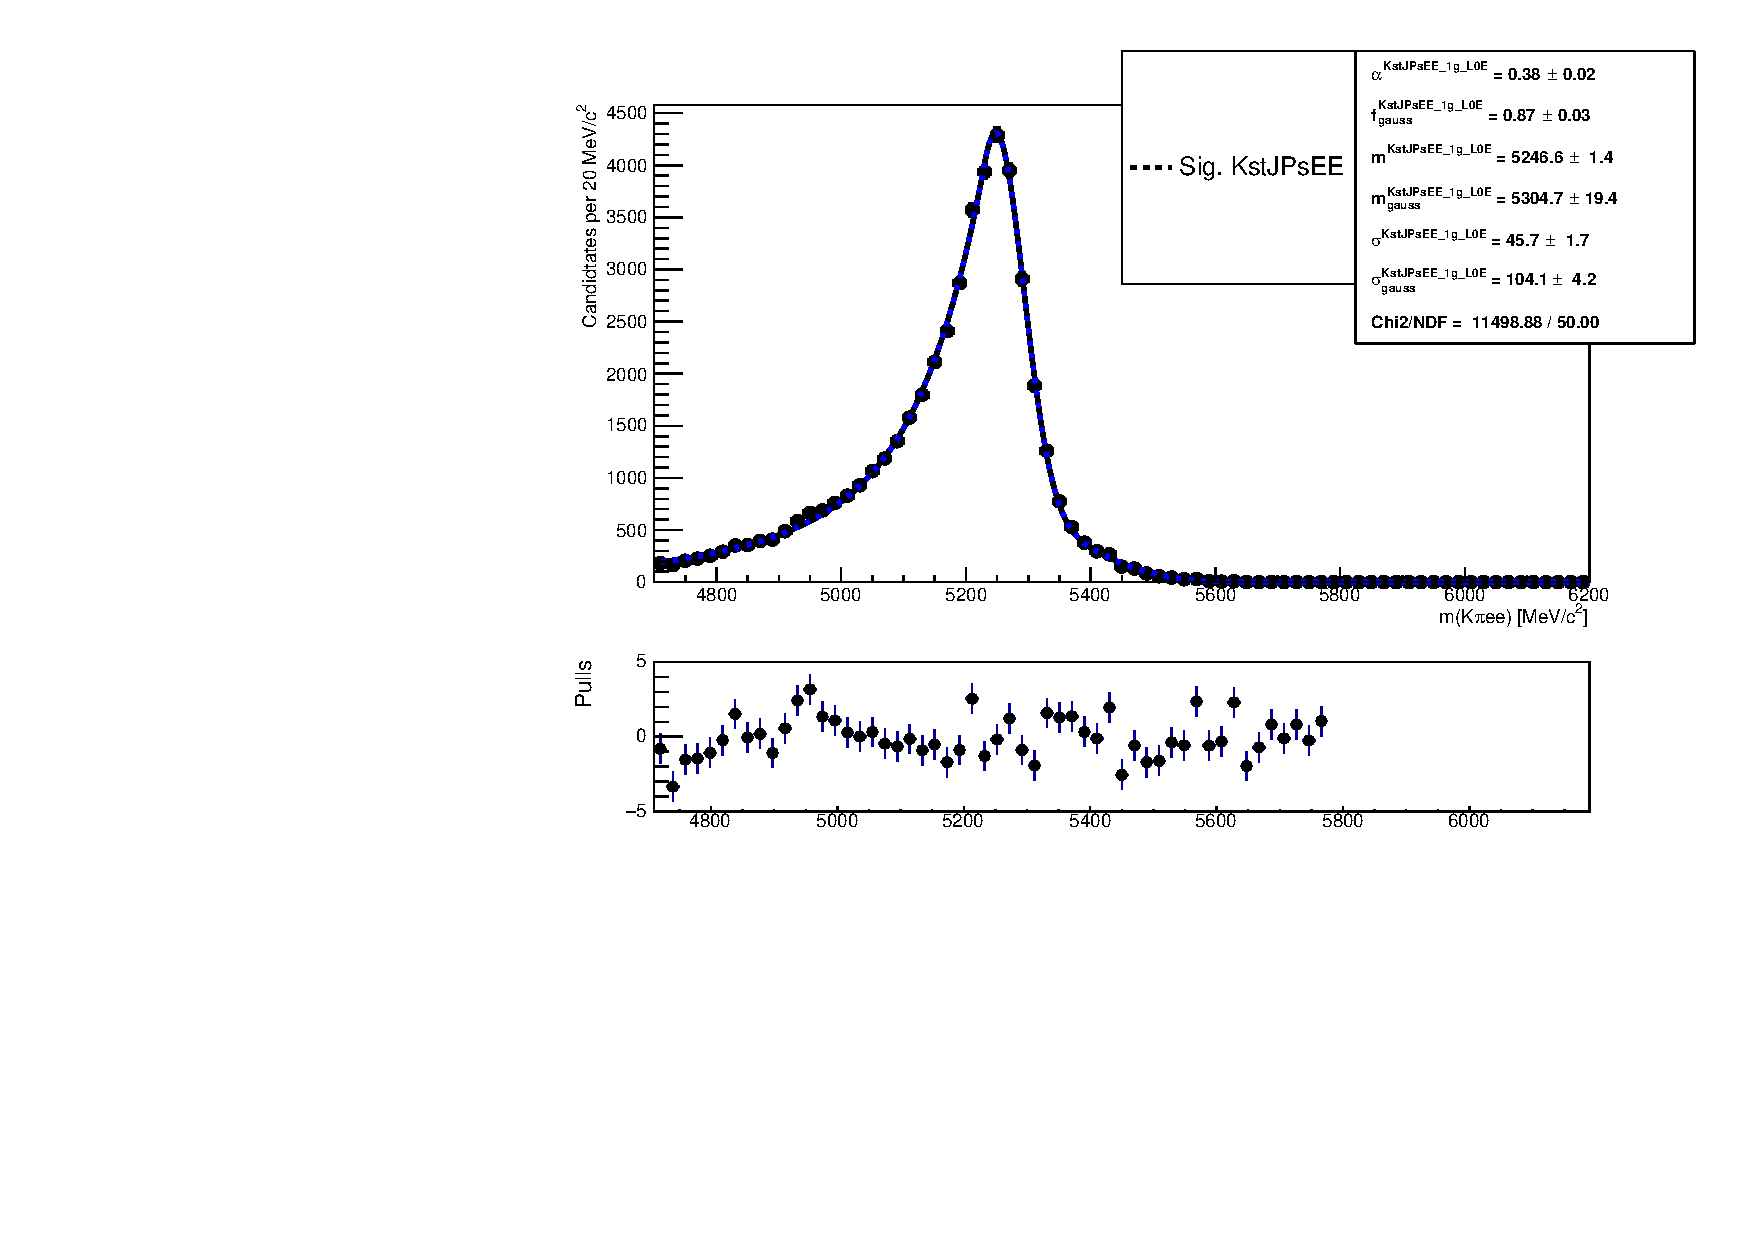
\includegraphics[width=0.6\textwidth]{RKst/figs/fit_EEs_0_EE-q2central-gmc/KstJPsEE_1g_L0E_fitAndRes.pdf}
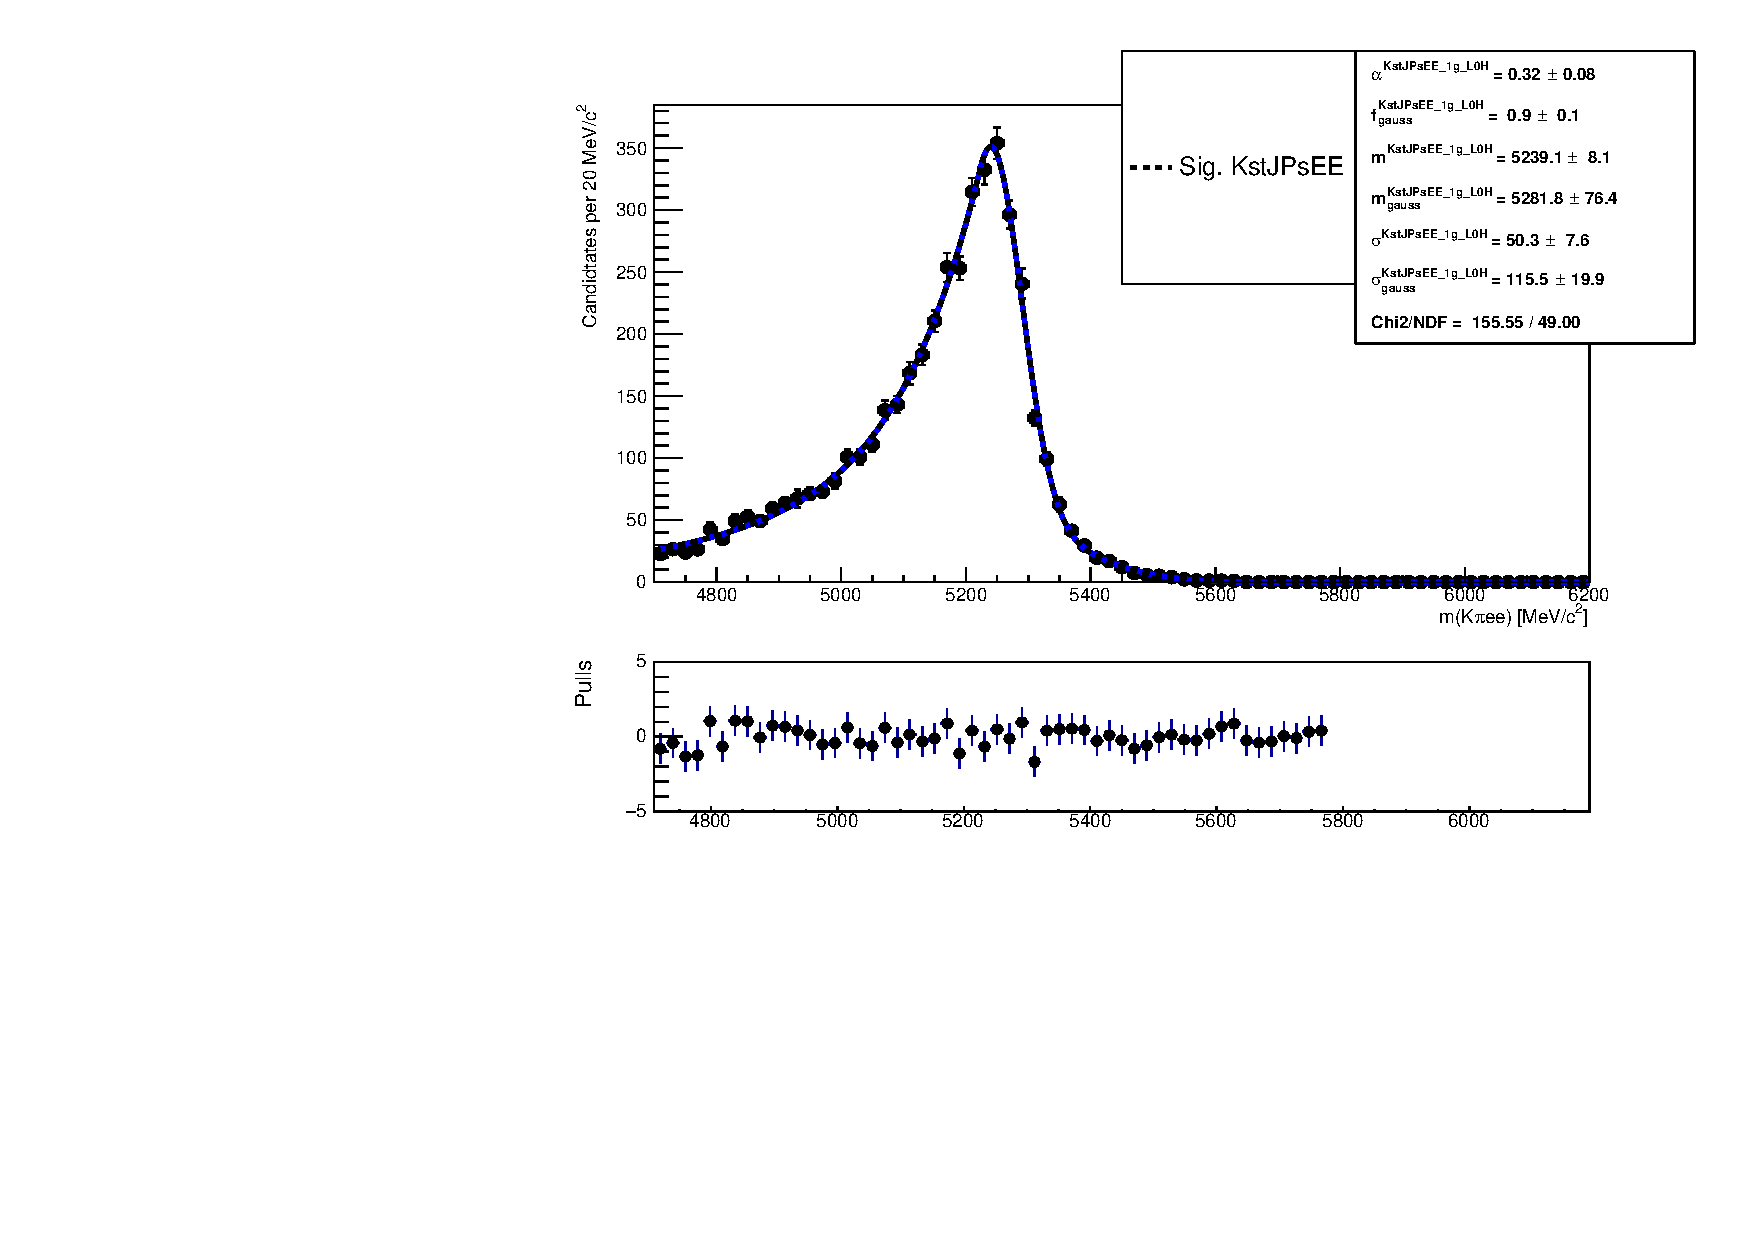
\includegraphics[width=0.6\textwidth]{RKst/figs/fit_EEs_0_EE-q2central-gmc/KstJPsEE_1g_L0H_fitAndRes.pdf}
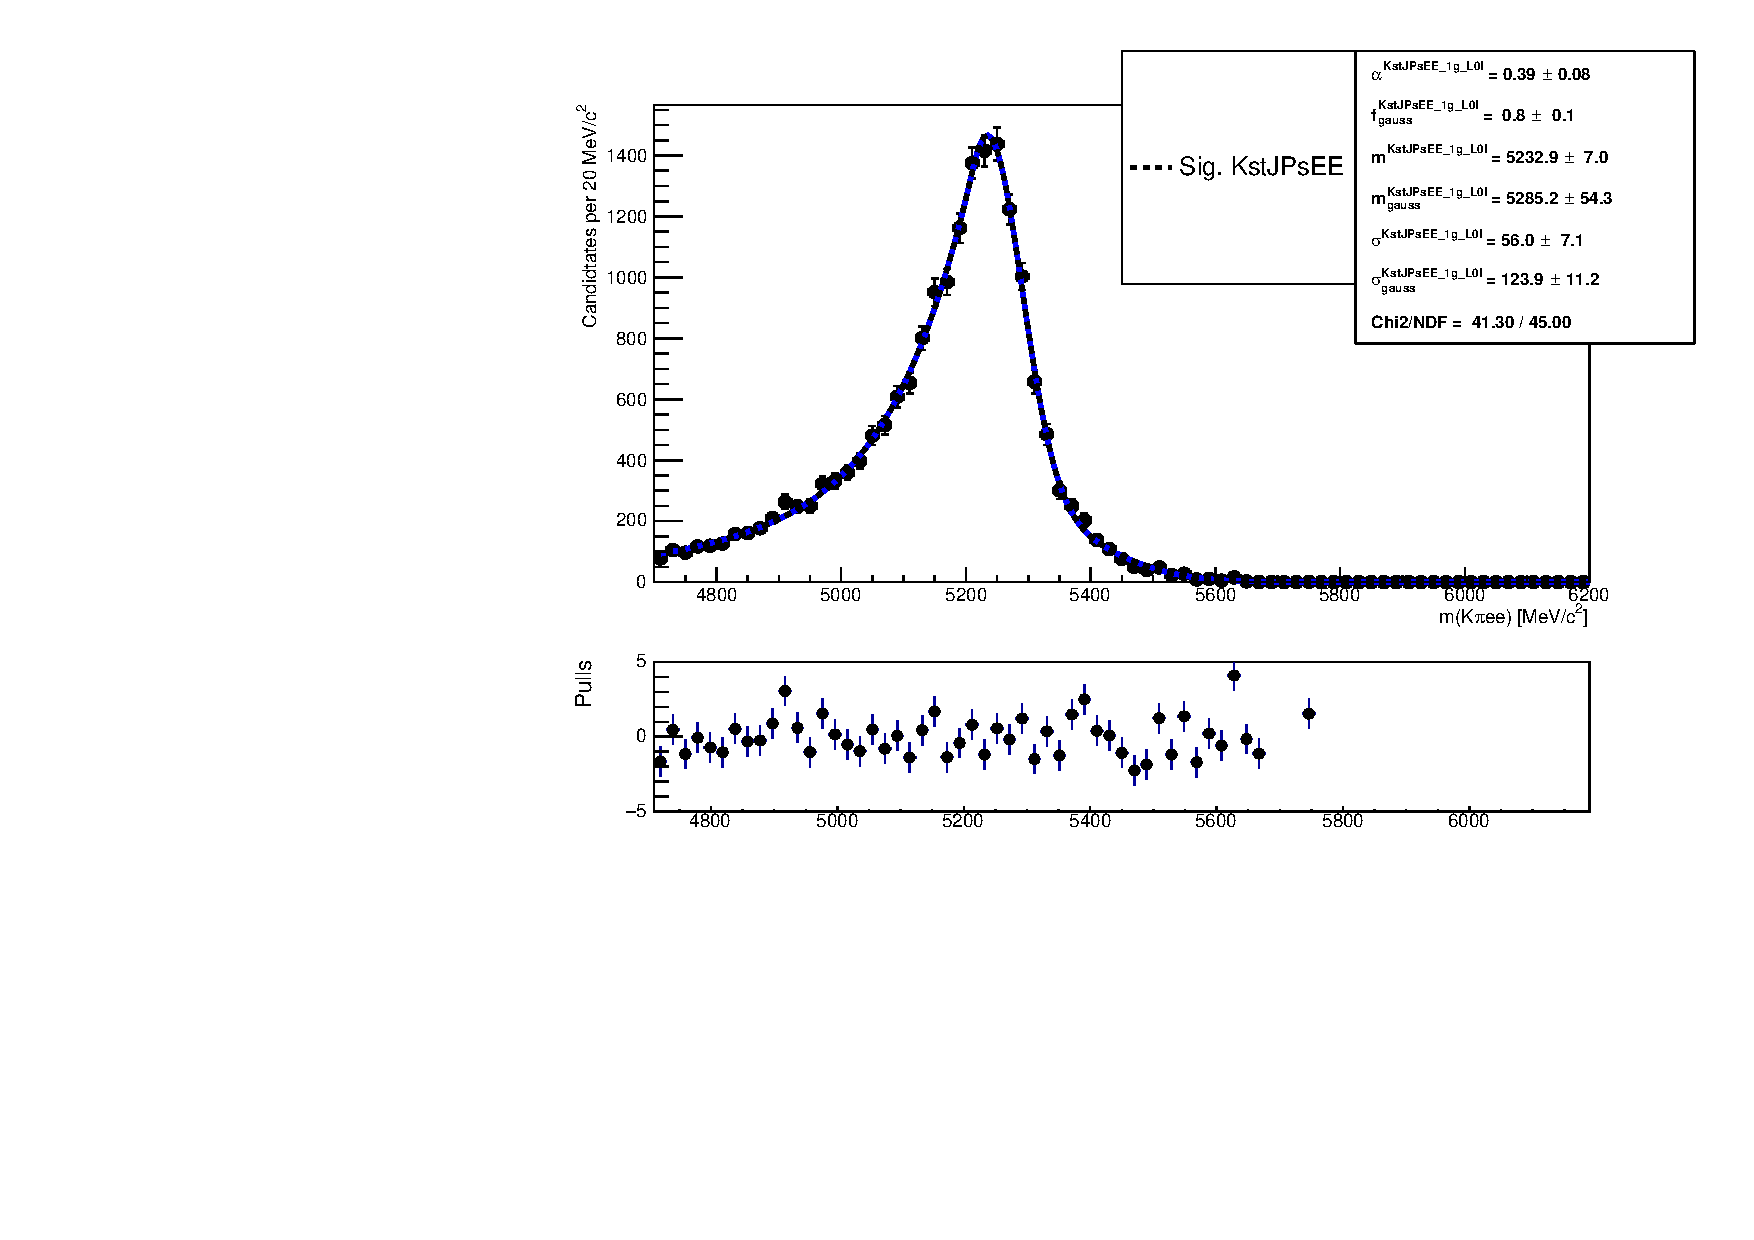
\includegraphics[width=0.6\textwidth]{RKst/figs/fit_EEs_0_EE-q2central-gmc/KstJPsEE_1g_L0I_fitAndRes.pdf}
\caption{Fitted $m(K\pi ee)$ mass spectrum of $B^0 \rightarrow K^{*0} J/\psi(J/\psi\rightarrow ee)$ simulated
events in the three trigger categories and one photon emitted. }
\label{fig:FitEE_MC_inTrigCat_Brem1}
\end{figure}
%
\begin{figure}[h!]
\centering
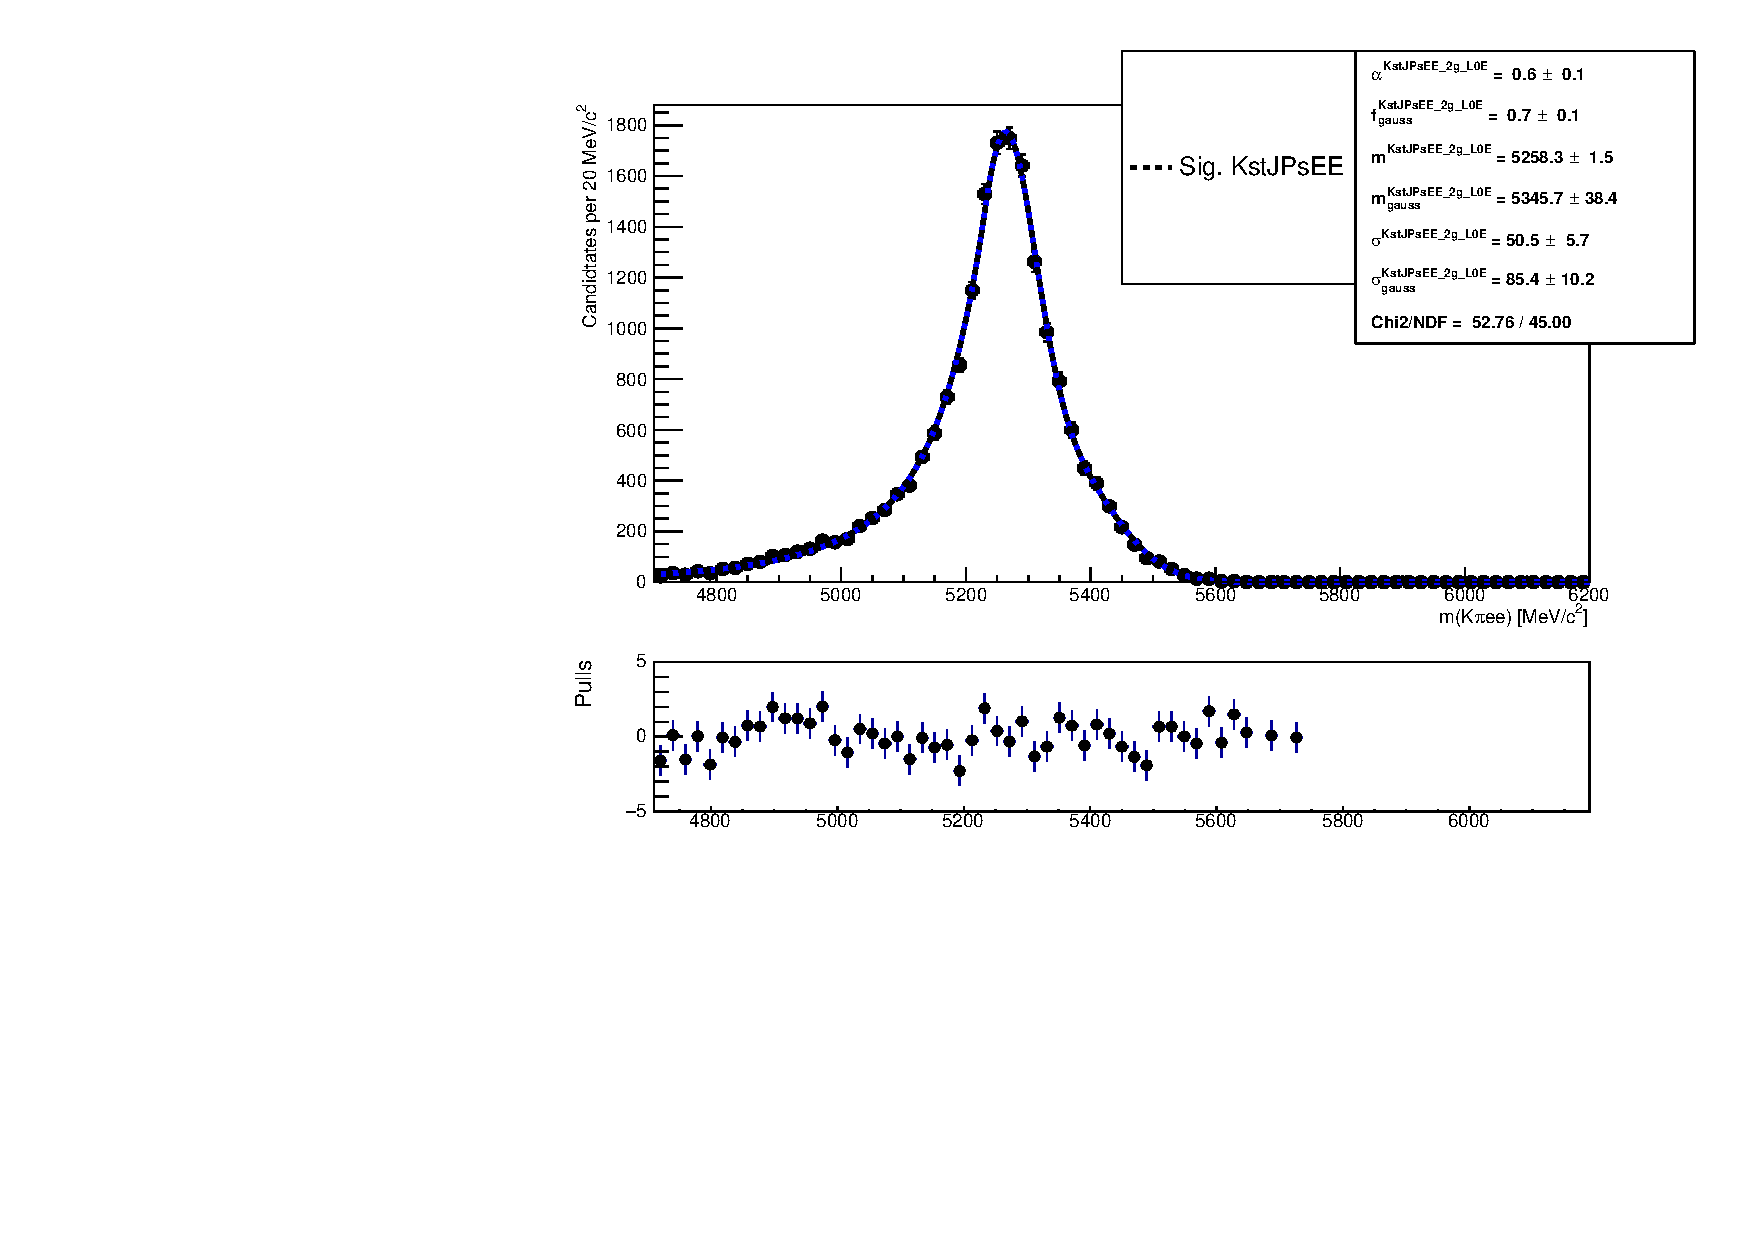
\includegraphics[width=0.6\textwidth]{RKst/figs/fit_EEs_0_EE-q2central-gmc/KstJPsEE_2g_L0E_fitAndRes.pdf}
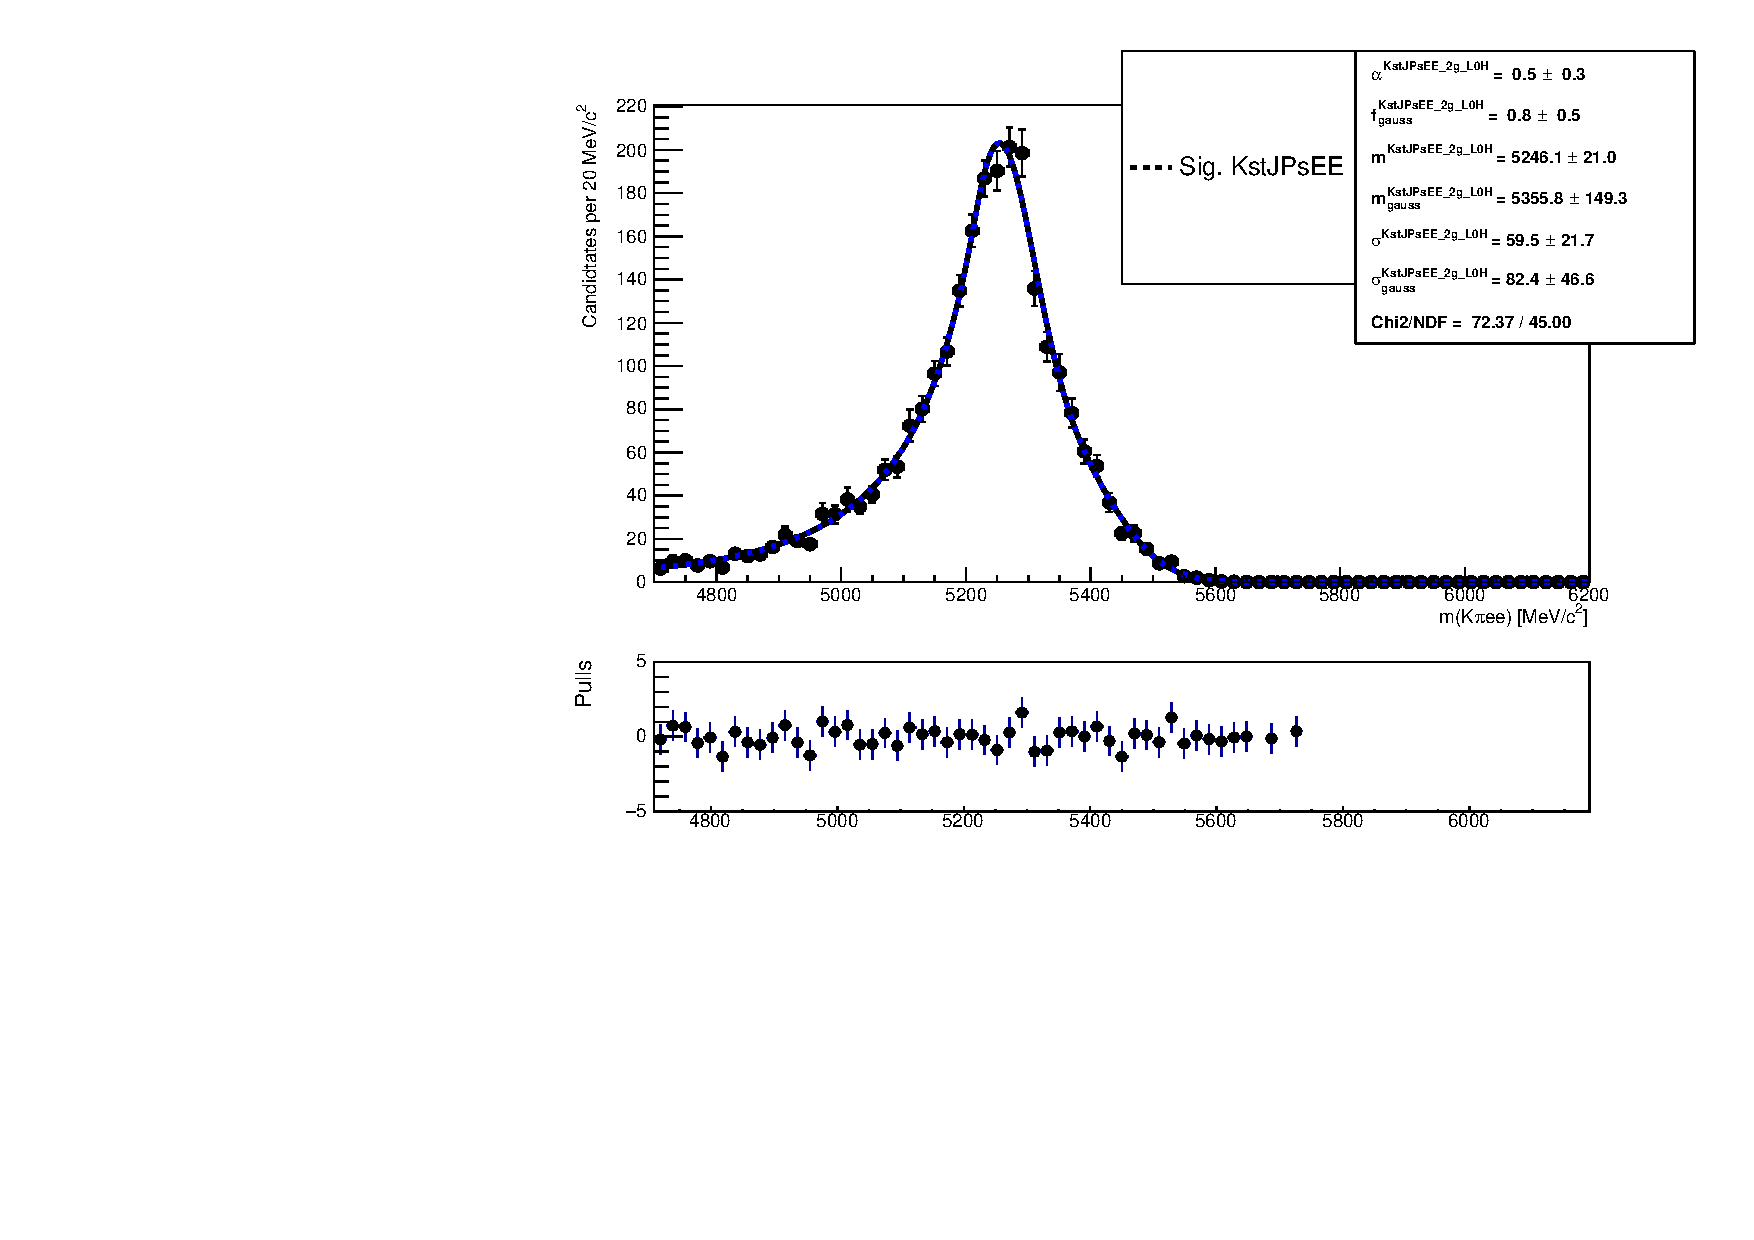
\includegraphics[width=0.6\textwidth]{RKst/figs/fit_EEs_0_EE-q2central-gmc/KstJPsEE_2g_L0H_fitAndRes.pdf}
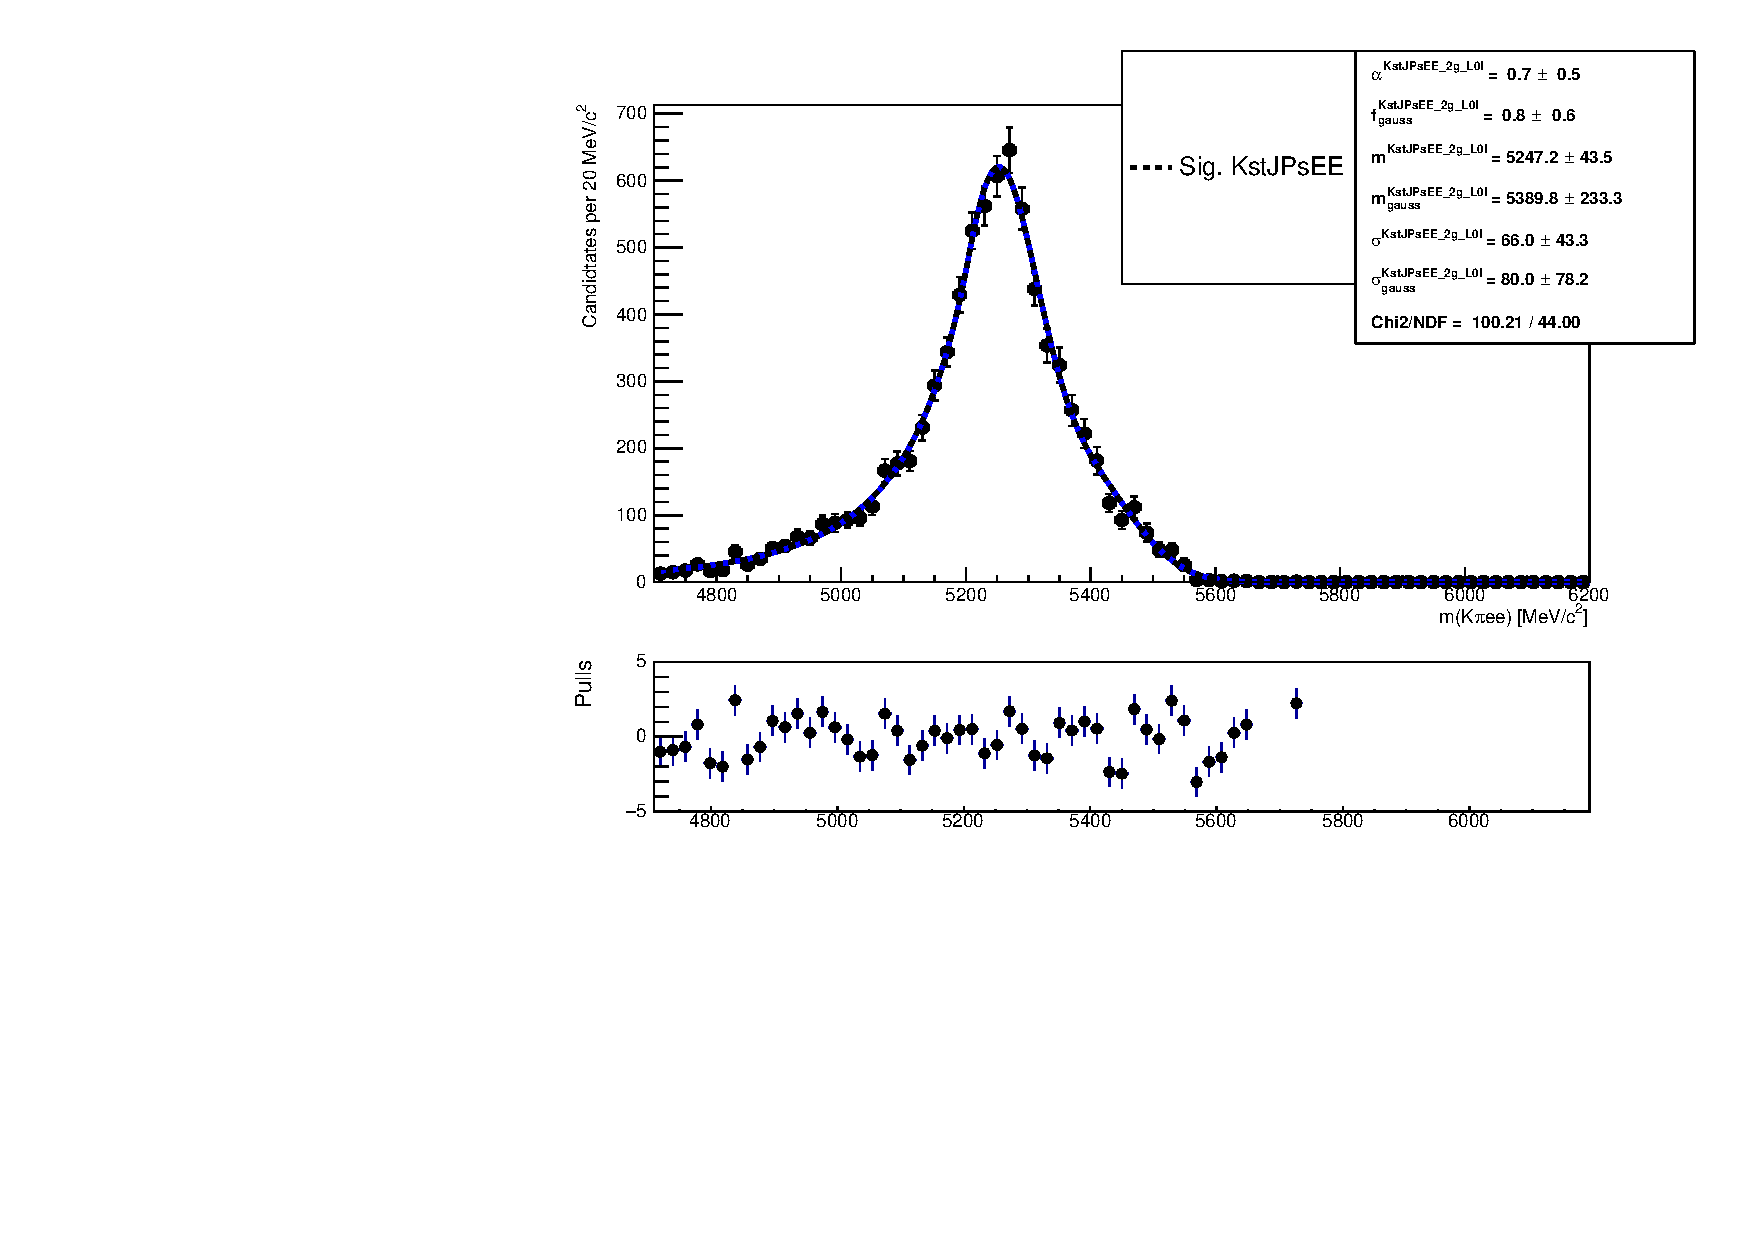
\includegraphics[width=0.6\textwidth]{RKst/figs/fit_EEs_0_EE-q2central-gmc/KstJPsEE_2g_L0I_fitAndRes.pdf}
\caption{Fitted $m(K\pi ee)$ mass spectrum of $B^0 \rightarrow K^{*0} J/\psi(J/\psi\rightarrow ee)$ simulated
events in the three trigger categories and two photons emitted. }
\label{fig:FitEE_MC_inTrigCat_Brem2}
\end{figure}

\chapter{Invariant mass fits to $\Bd\to\Kstarz\ee$ candidates divided in trigger categories}
\label{app:RKDatafits}

This appendix contains fits to the $m(K\pi ee )$ invariant mass of rare and control channel
candidates separately in the tree trigger categories. Each trigger category is always fit
with its own PDF but in the main text only their sum is shown for simplicity.

\begin{figure}[h!]
\centering
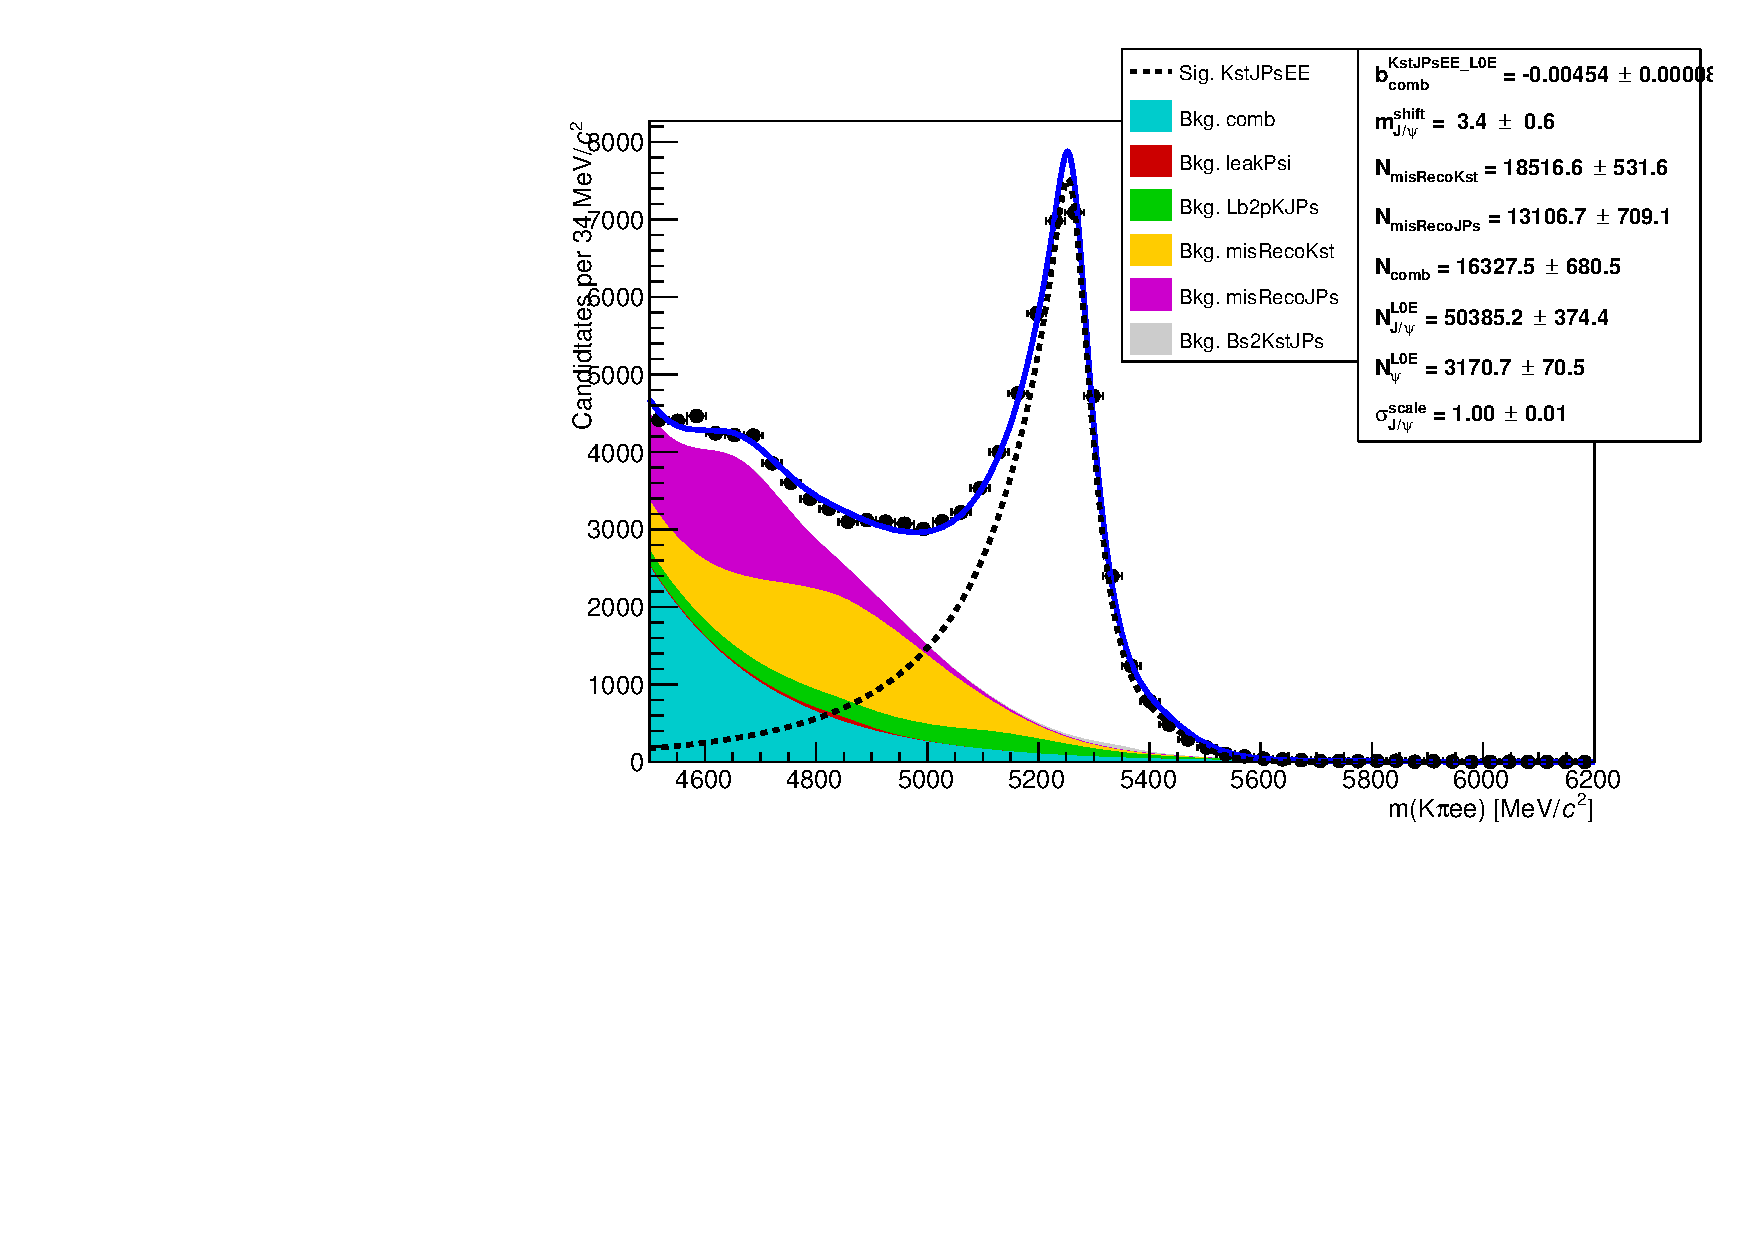
\includegraphics[width=0.49\textwidth]{RKst/figs/Fit/fit_EE/KstJPsEE_L0E.pdf}
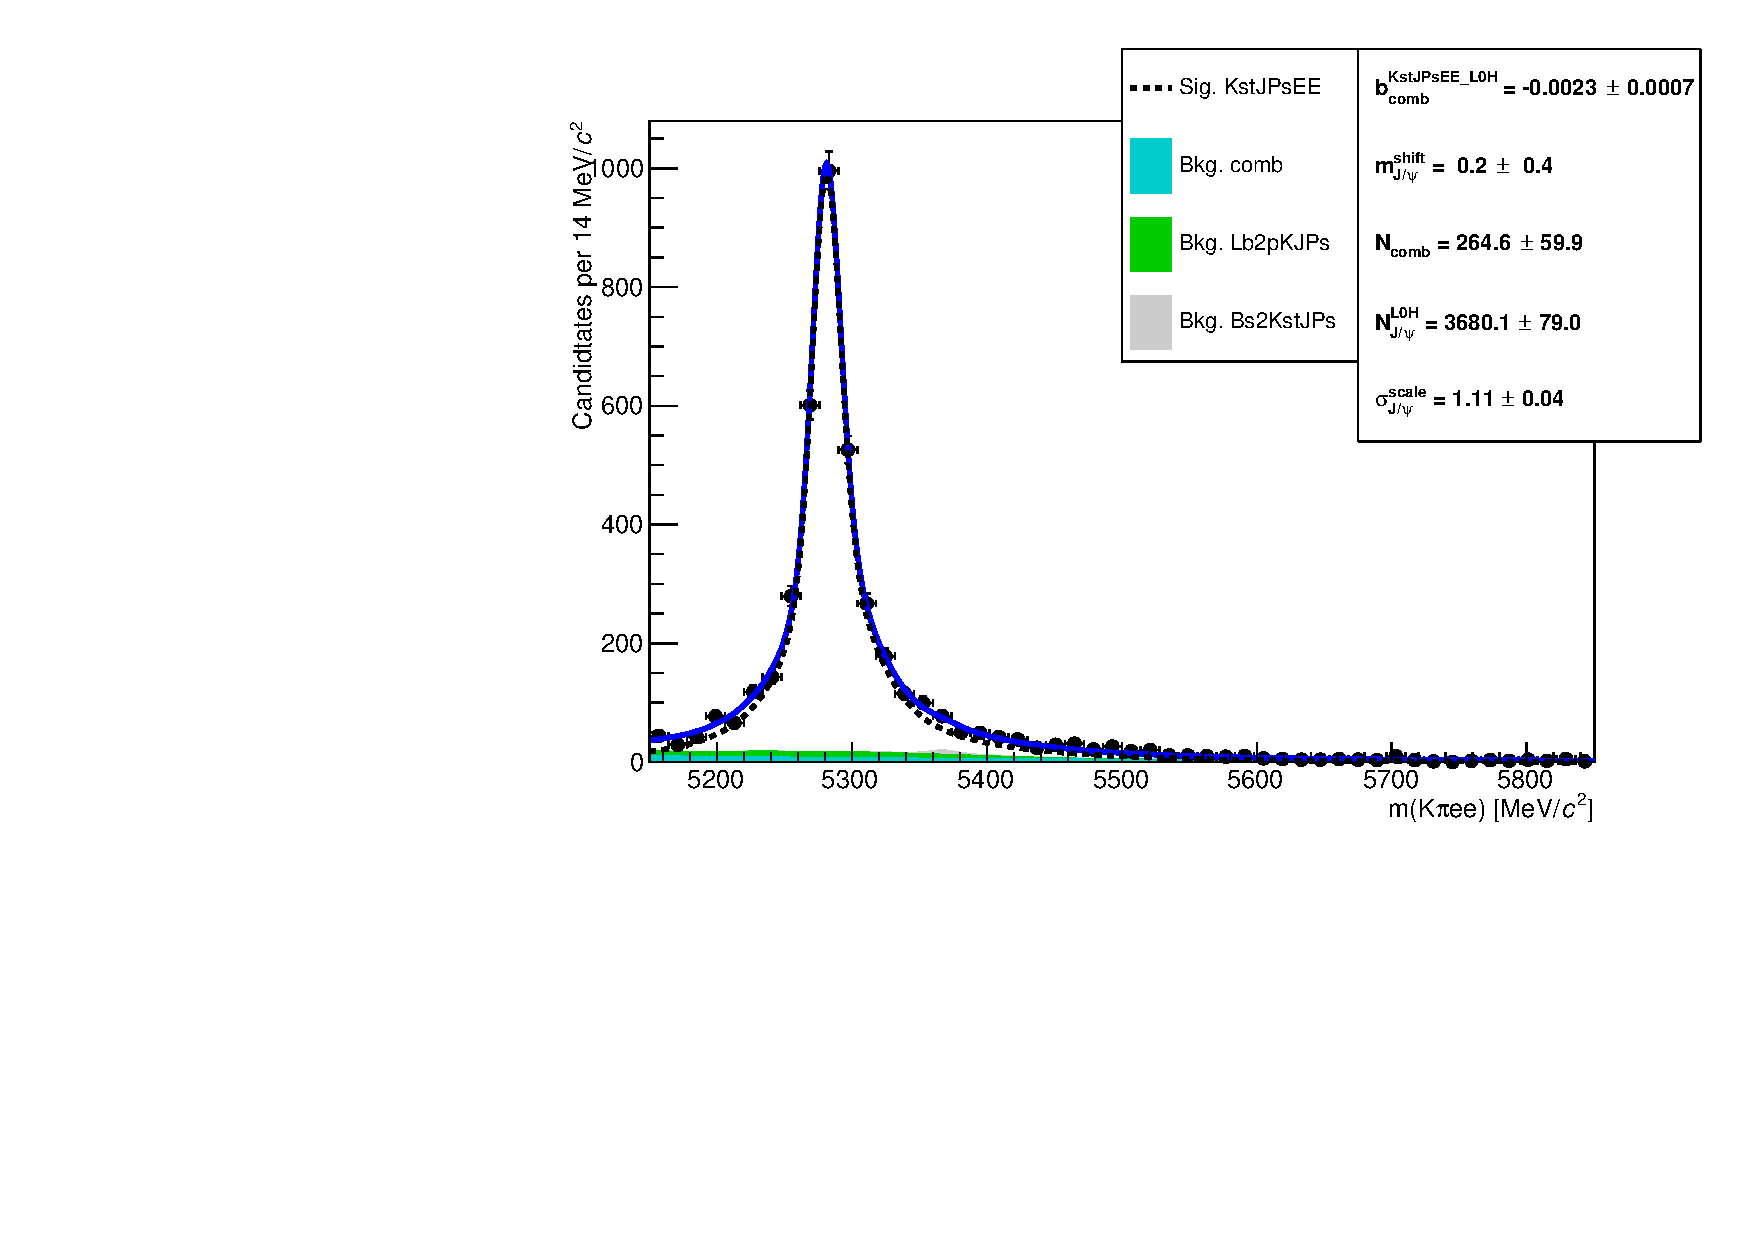
\includegraphics[width=0.49\textwidth]{RKst/figs/Fit/fit_EE/KstJPsEE_L0H.pdf}
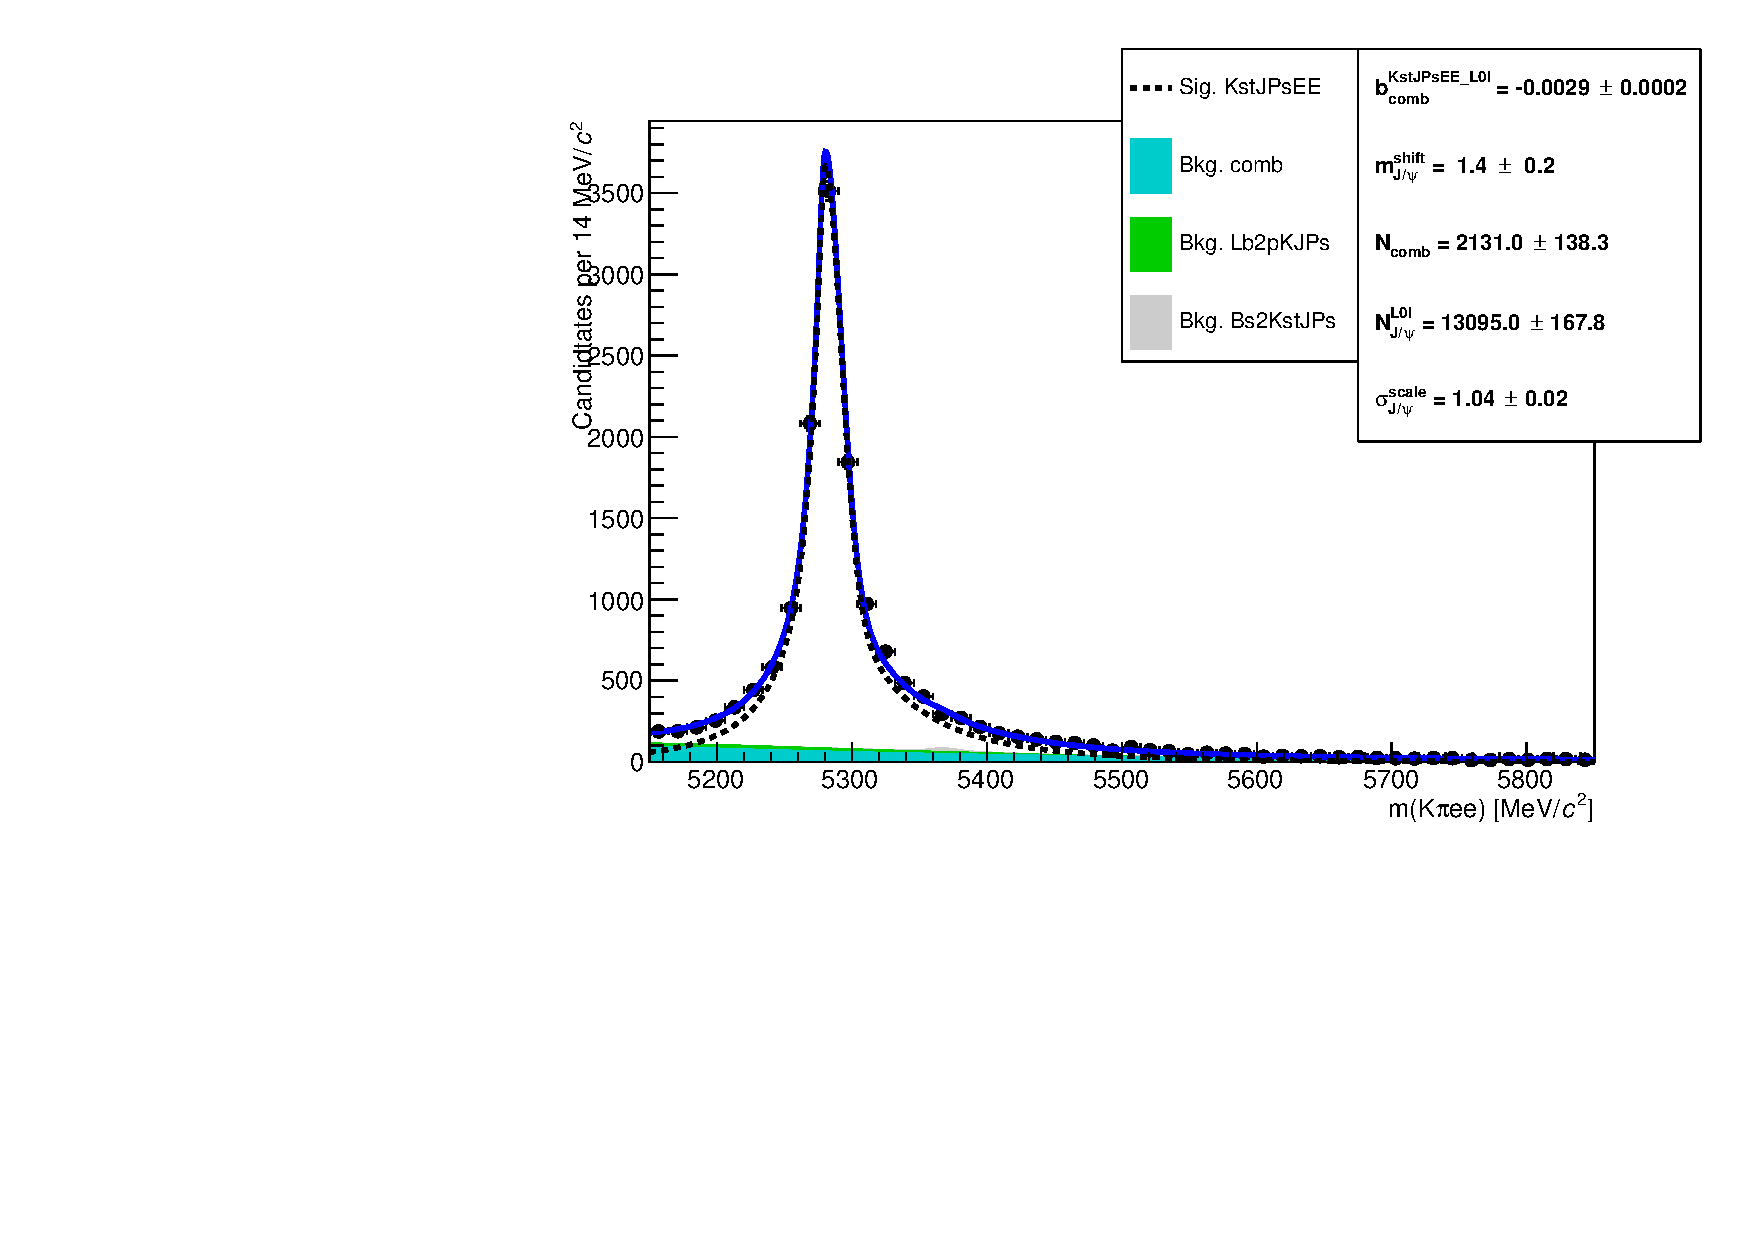
\includegraphics[width=0.49\textwidth]{RKst/figs/Fit/fit_EE/KstJPsEE_L0I.pdf}
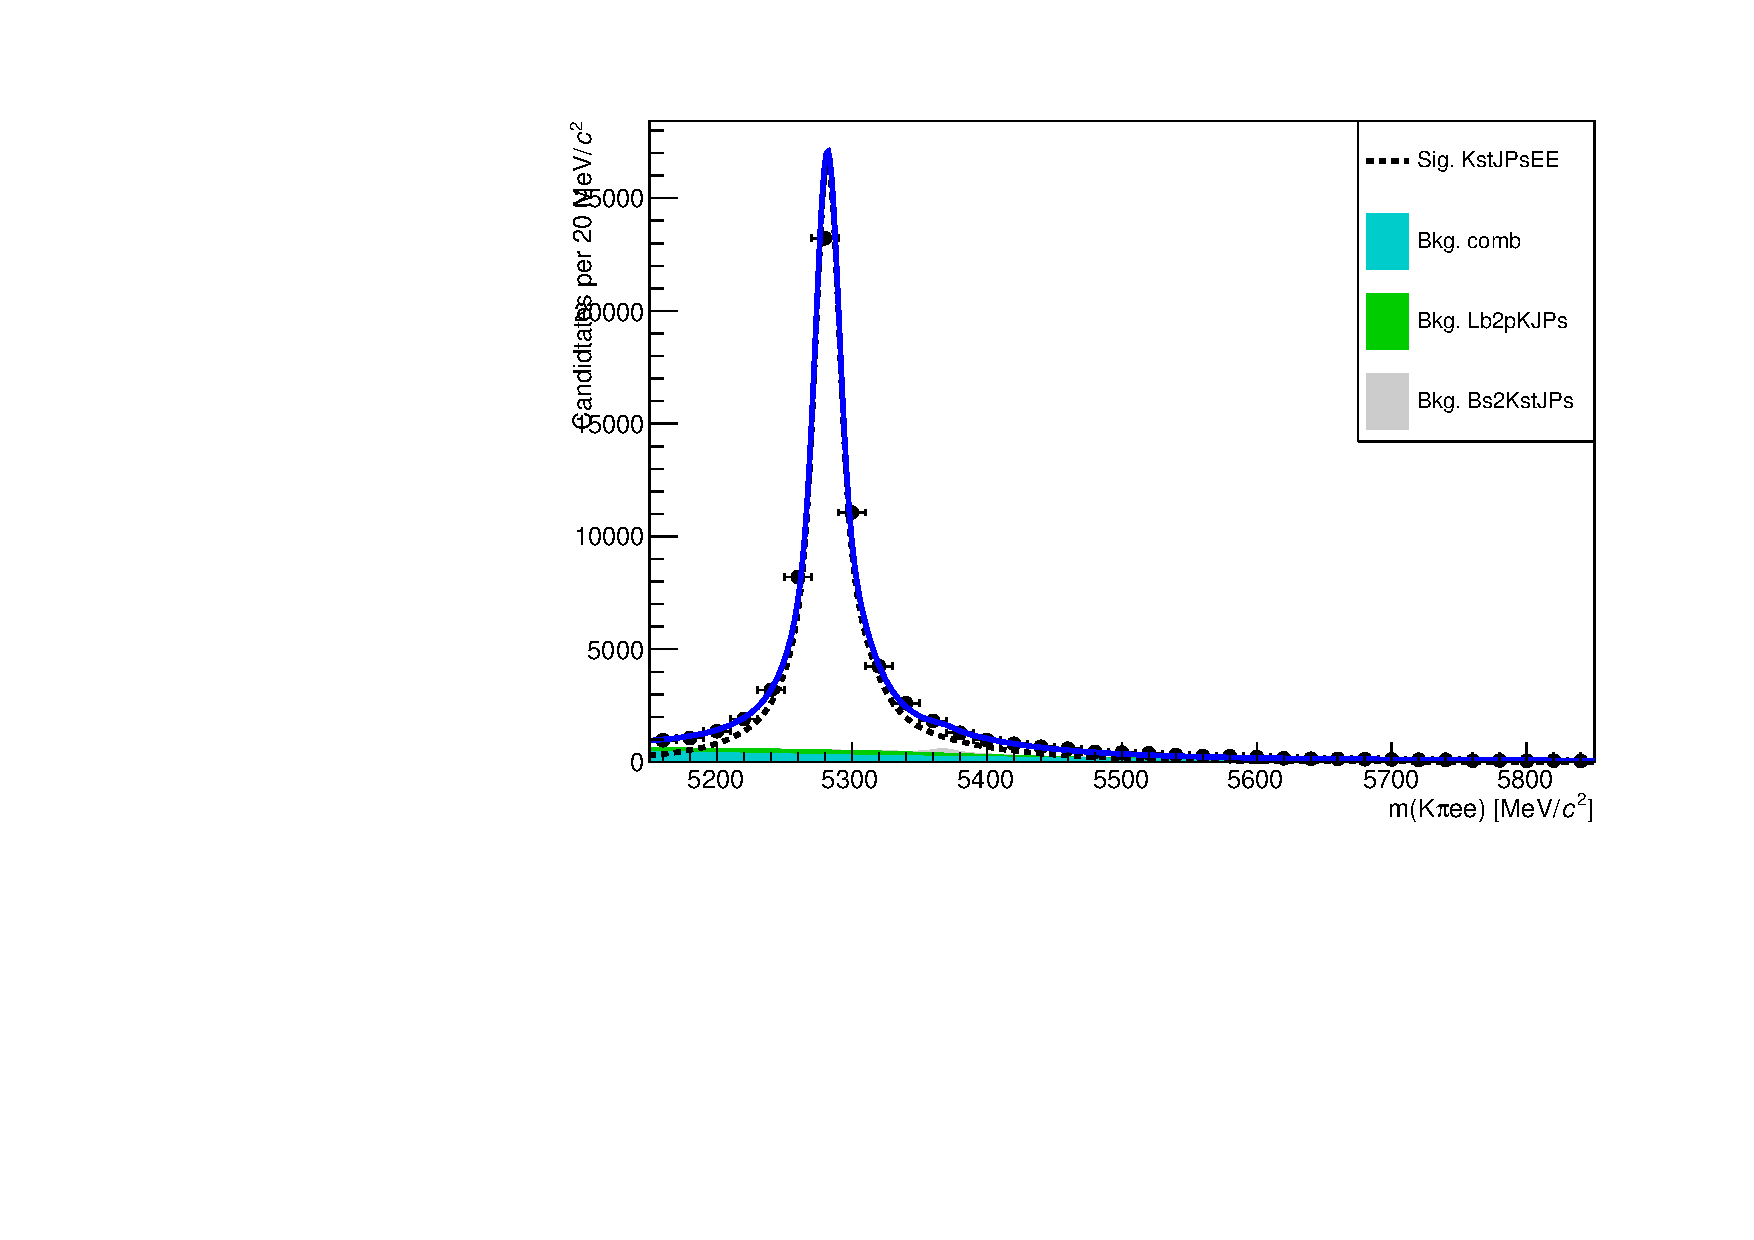
\includegraphics[width=0.49\textwidth]{RKst/figs/Fit/fit_EE/fit_JPs_L.pdf}
\caption{Fit to the \mKpiee invariant mass of \BdToKstJPsee candidates in the three trigger categories 
(L0E, L0H and L0I) separately, and (bottom right) combined. The dashed black line (shaded shapes) 
represents the signal (background) PDF.}
\label{fig:fitJPs_control_EE}
\end{figure}
%
\begin{figure}[h!]
\centering
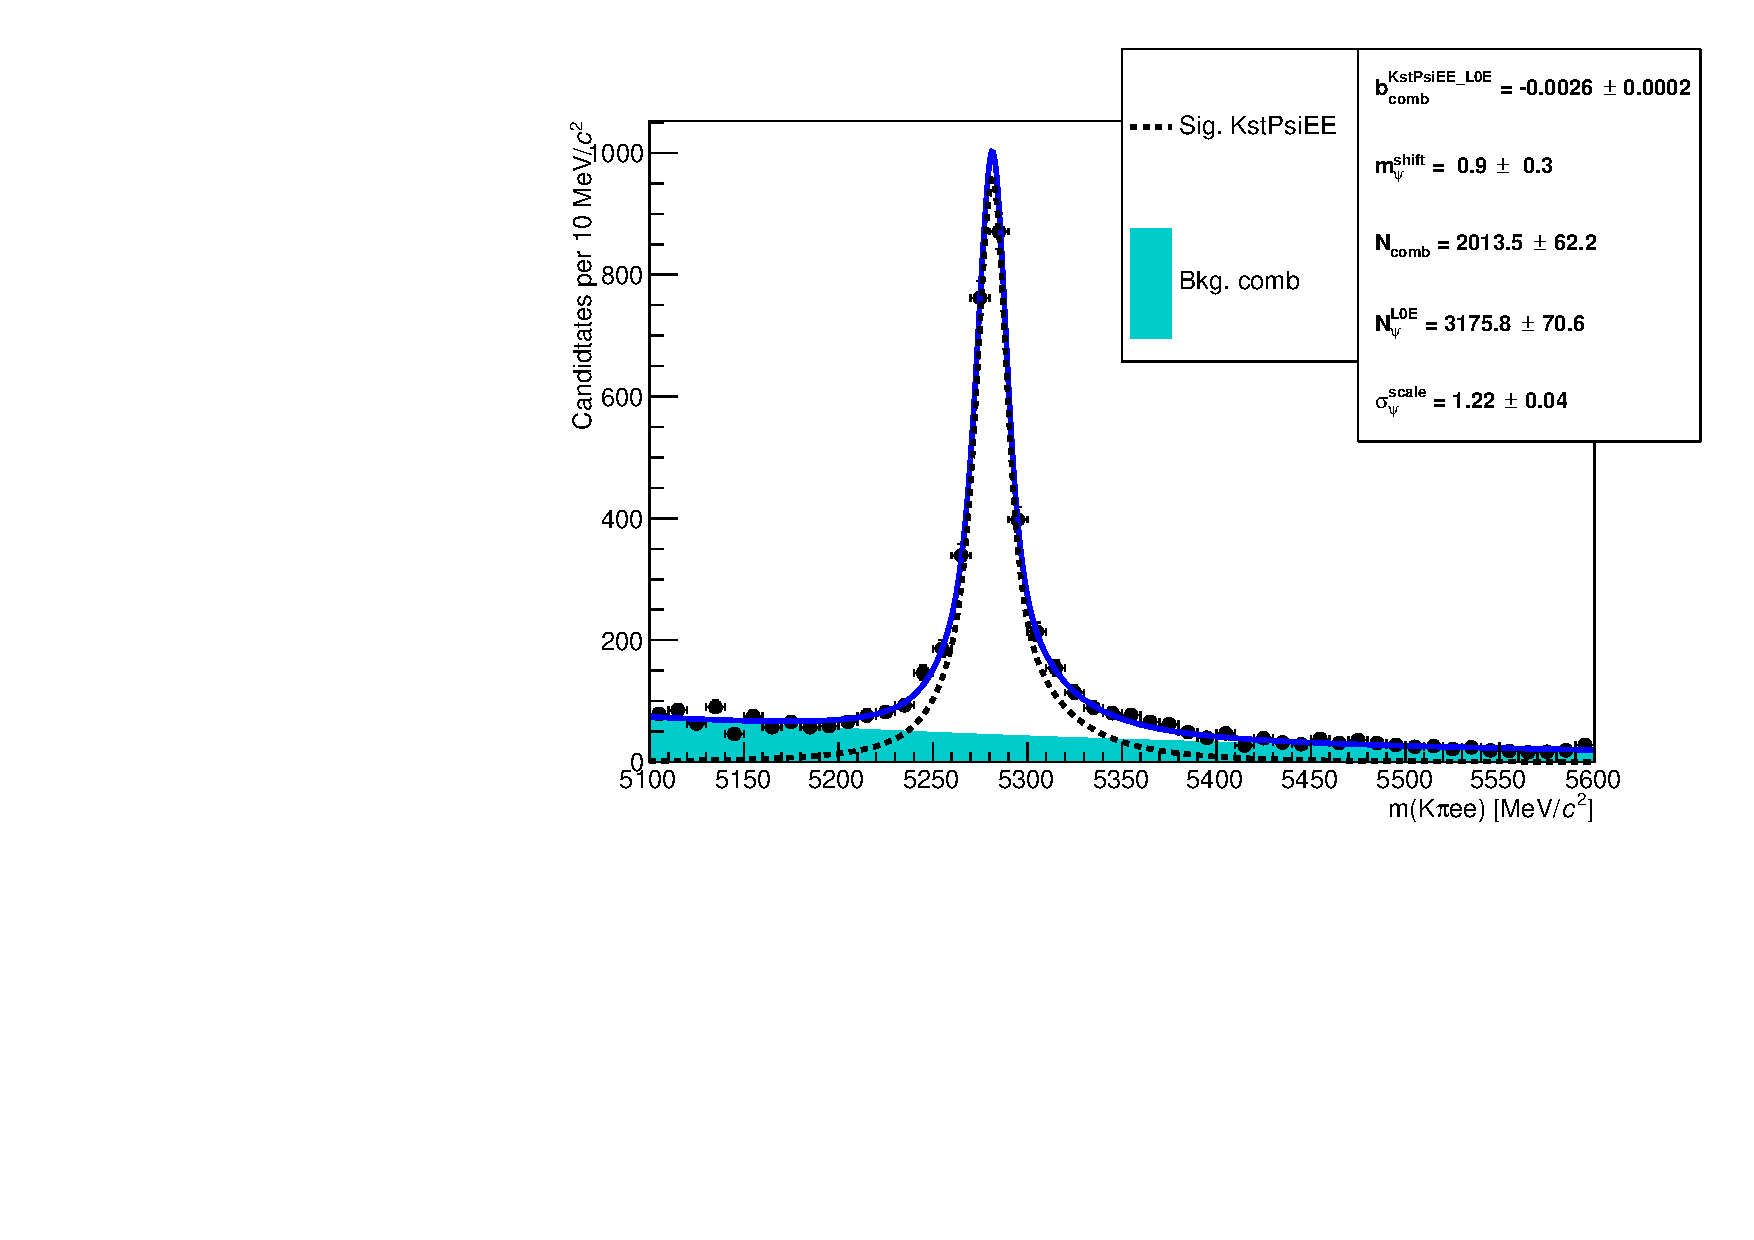
\includegraphics[width=0.49\textwidth]{RKst/figs/Fit/fit_EE/KstPsiEE_L0E.pdf}
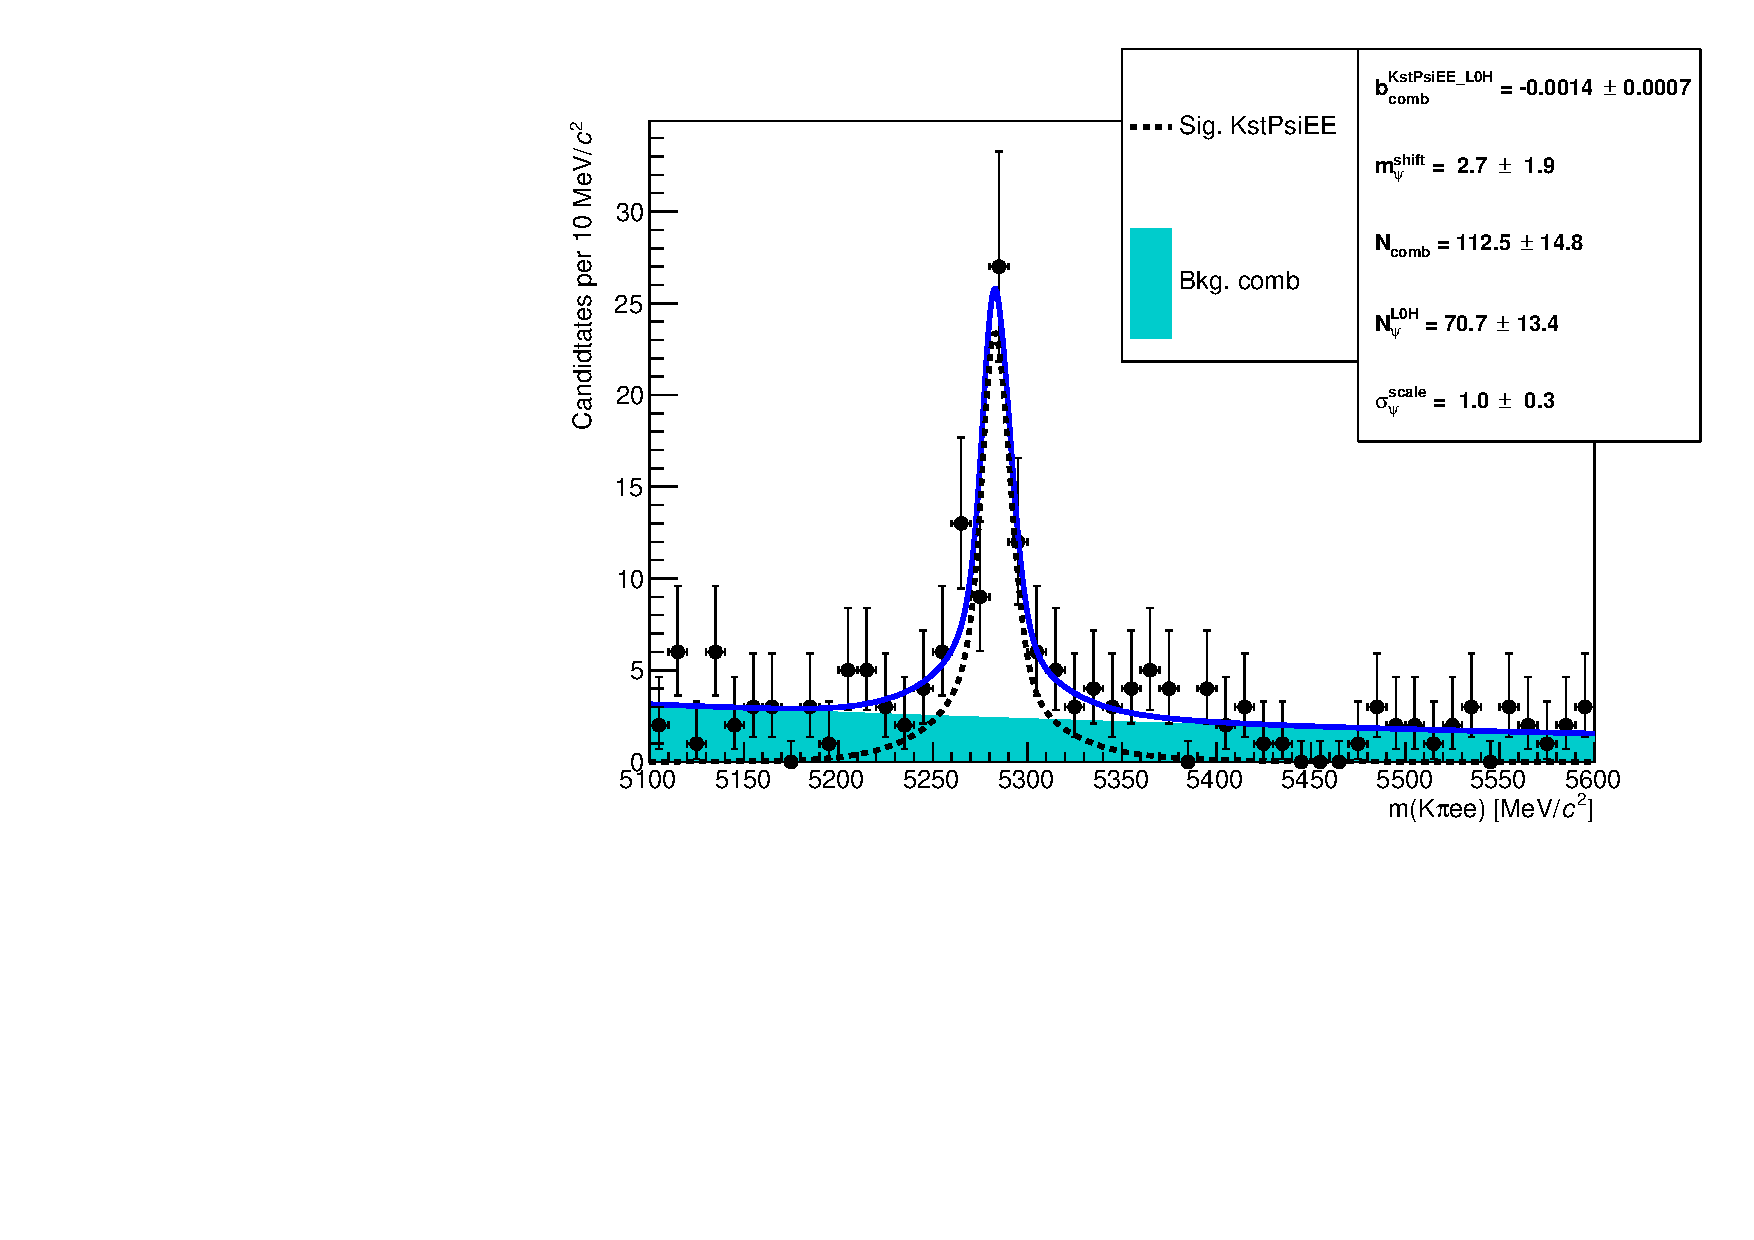
\includegraphics[width=0.49\textwidth]{RKst/figs/Fit/fit_EE/KstPsiEE_L0H.pdf}
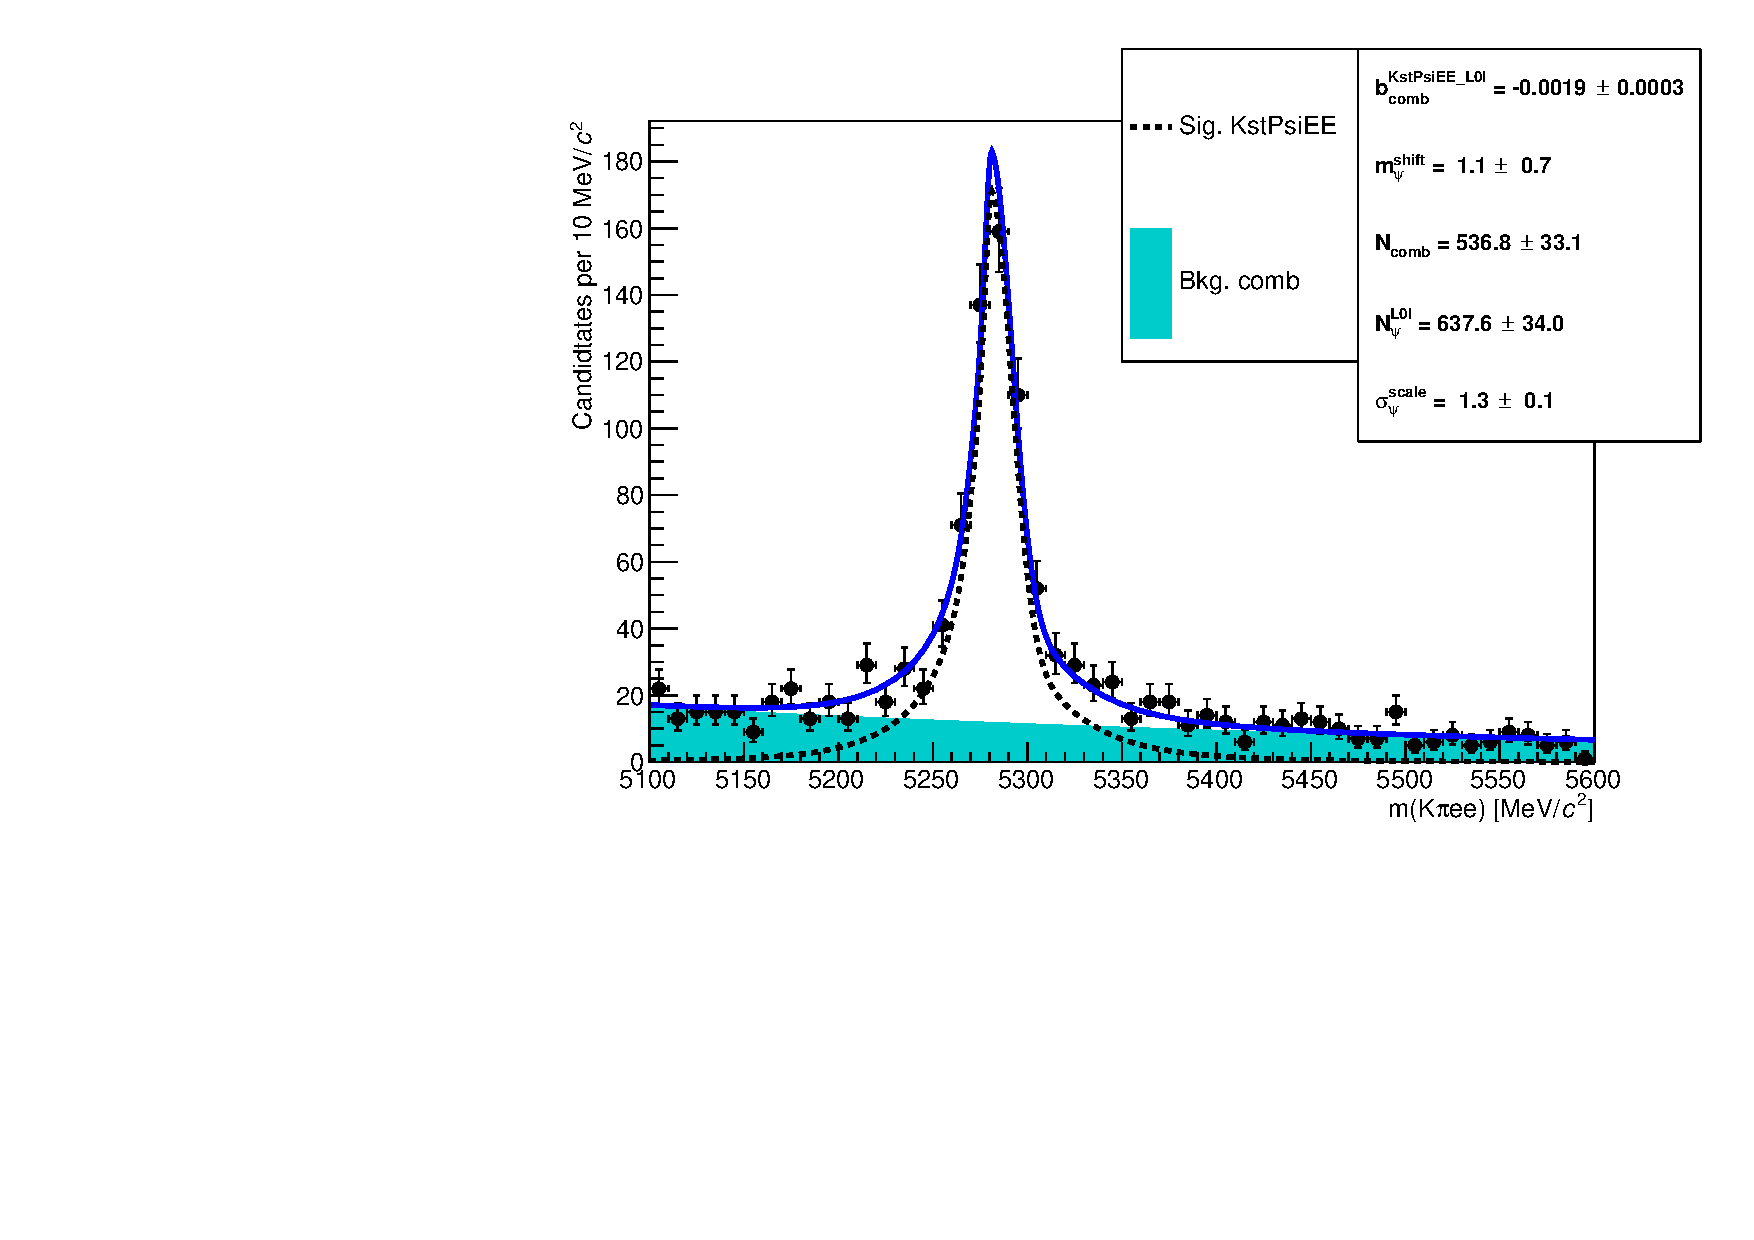
\includegraphics[width=0.49\textwidth]{RKst/figs/Fit/fit_EE/KstPsiEE_L0I.pdf}
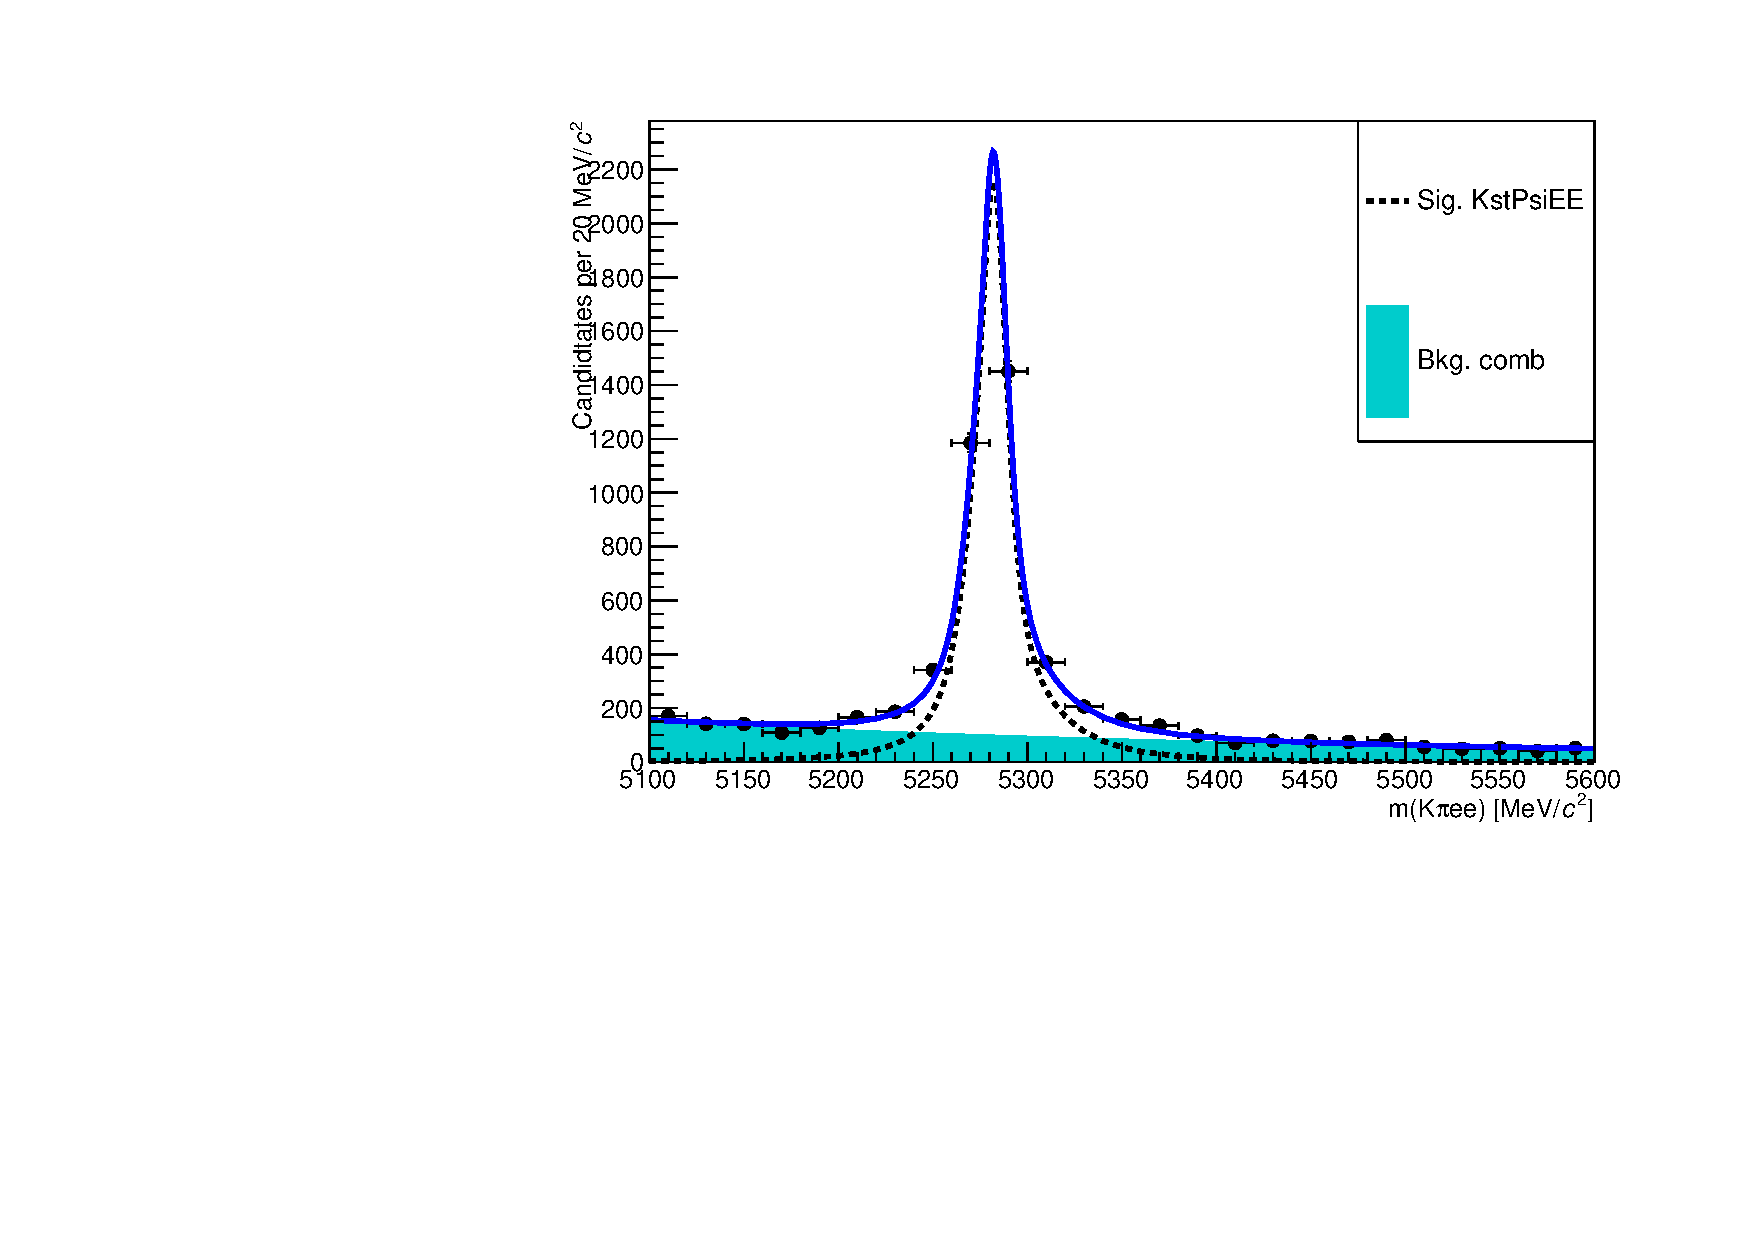
\includegraphics[width=0.49\textwidth]{RKst/figs/Fit/fit_EE/fit_Psi.pdf}
\caption{Fit to the \mKpiee invariant mass of $\Bd\to\Kstarz(\psitwos\to\ee)$ candidates in the three trigger categories (L0E, L0H and L0I) separately, and (bottom right) combined. The dashed black line (shaded shapes) represents the signal (background) PDF.}
\label{fig:fitPsiEE}
\end{figure}
%
\begin{figure}[h!]
\centering
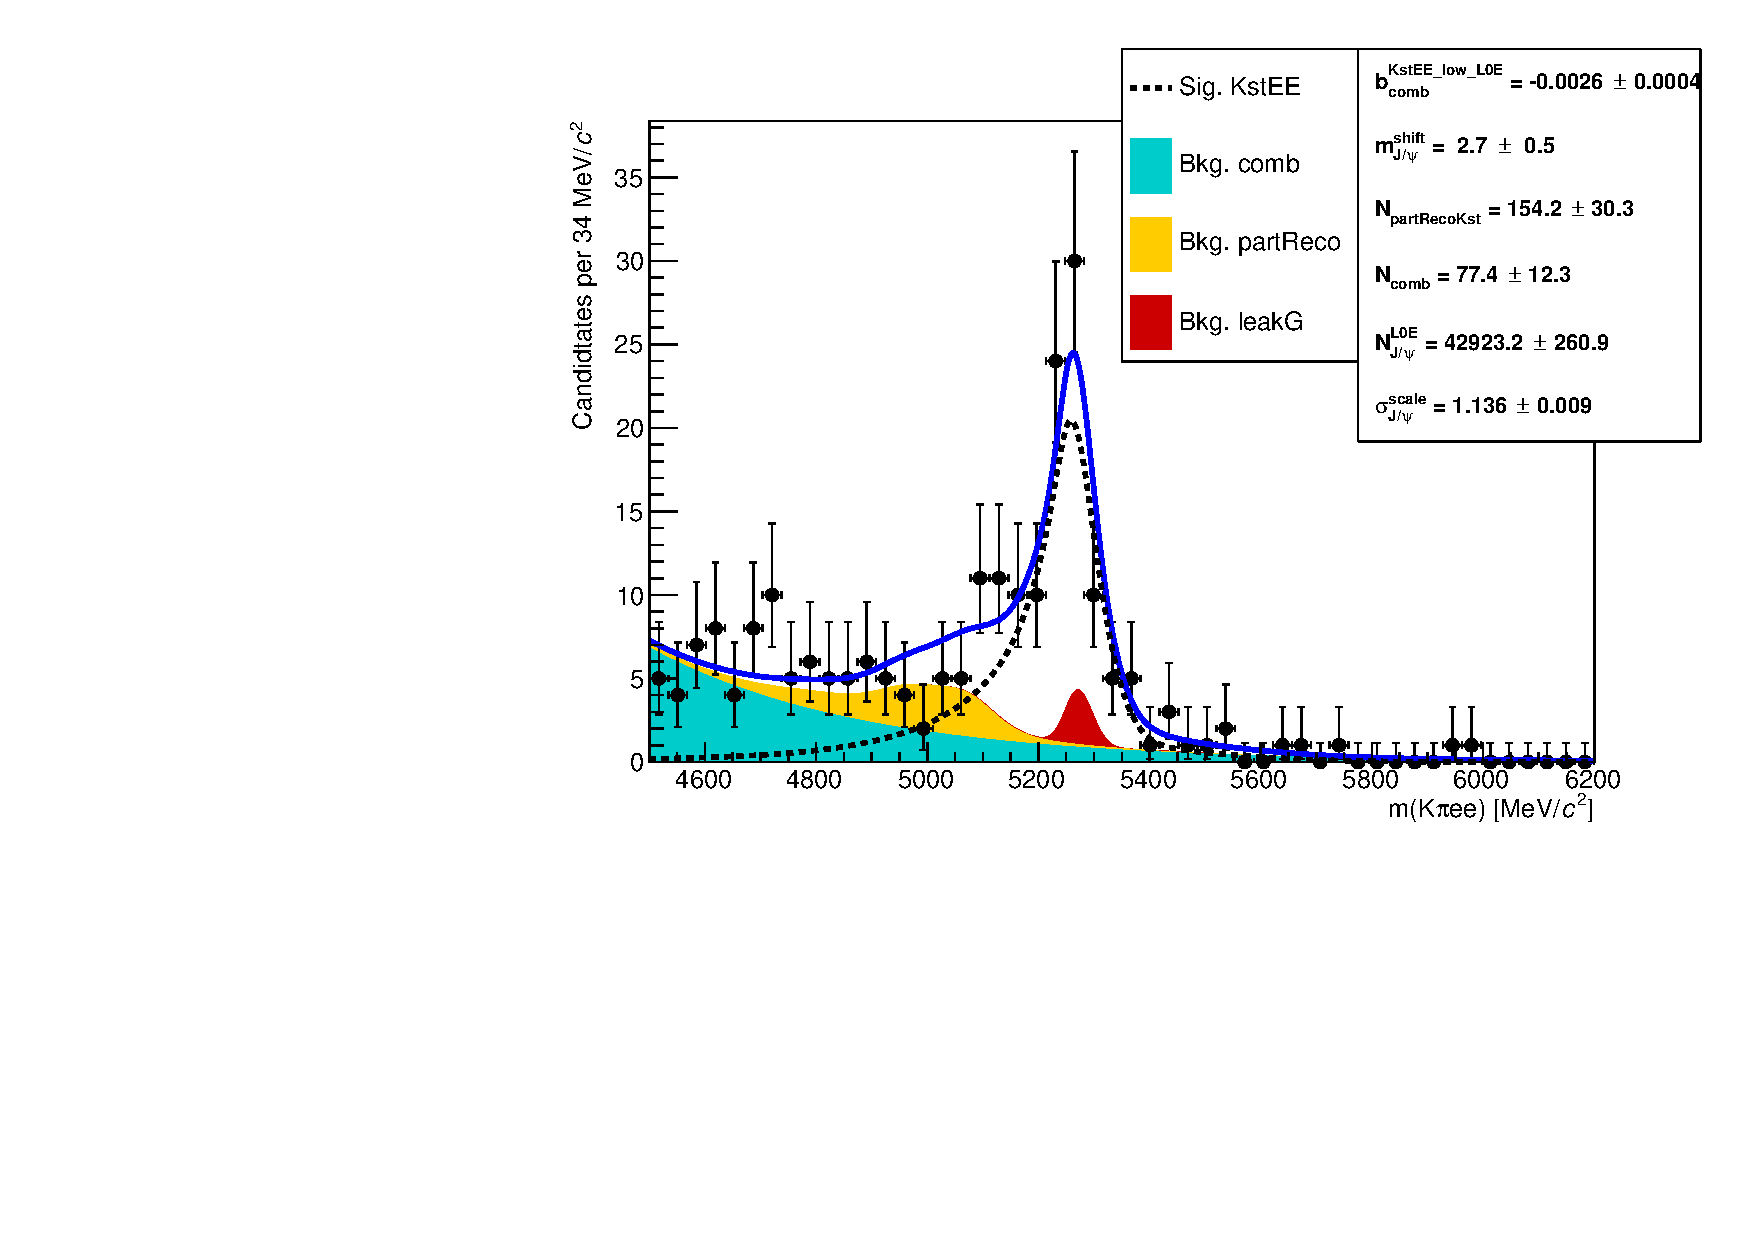
\includegraphics[width=0.49\textwidth]{RKst/figs/Fit/fit_EE/KstEE_low_L0E.pdf}
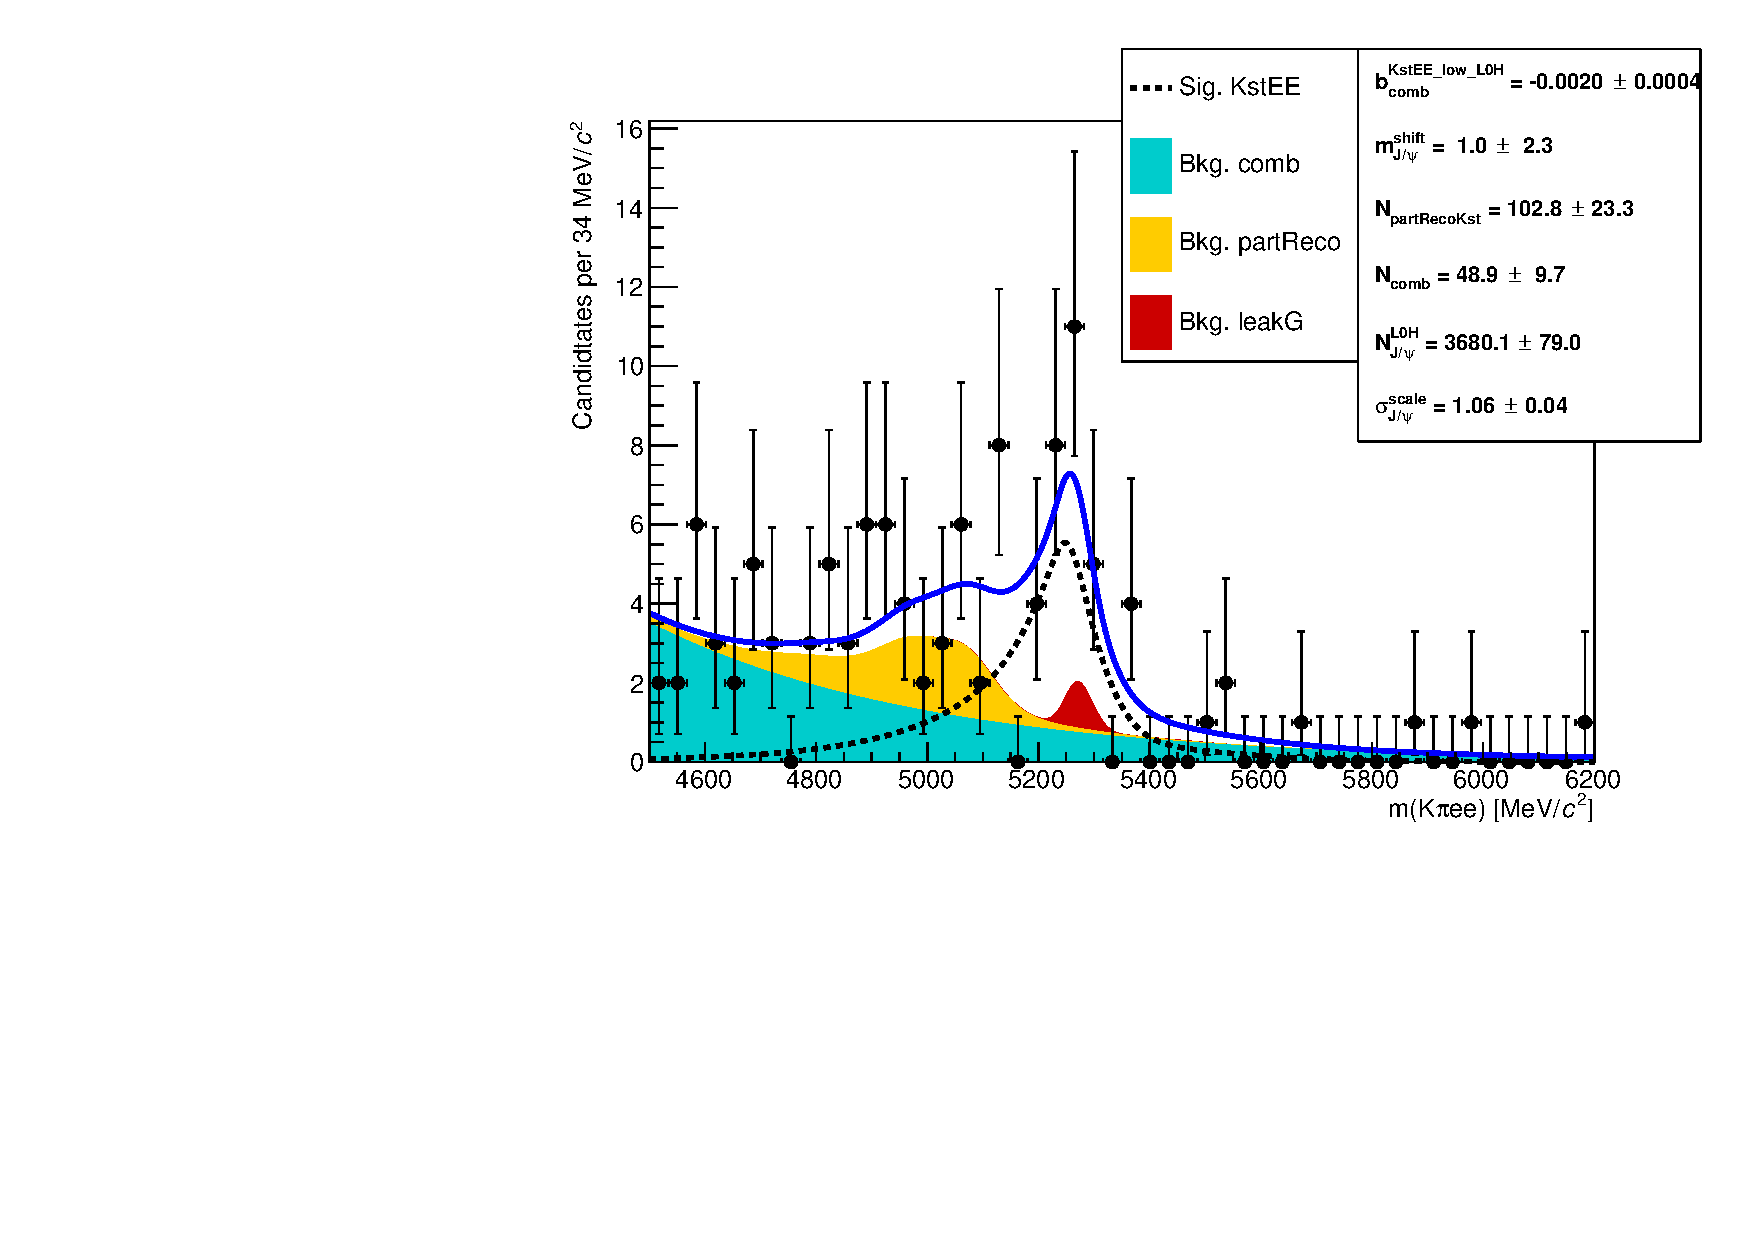
\includegraphics[width=0.49\textwidth]{RKst/figs/Fit/fit_EE/KstEE_low_L0H.pdf}
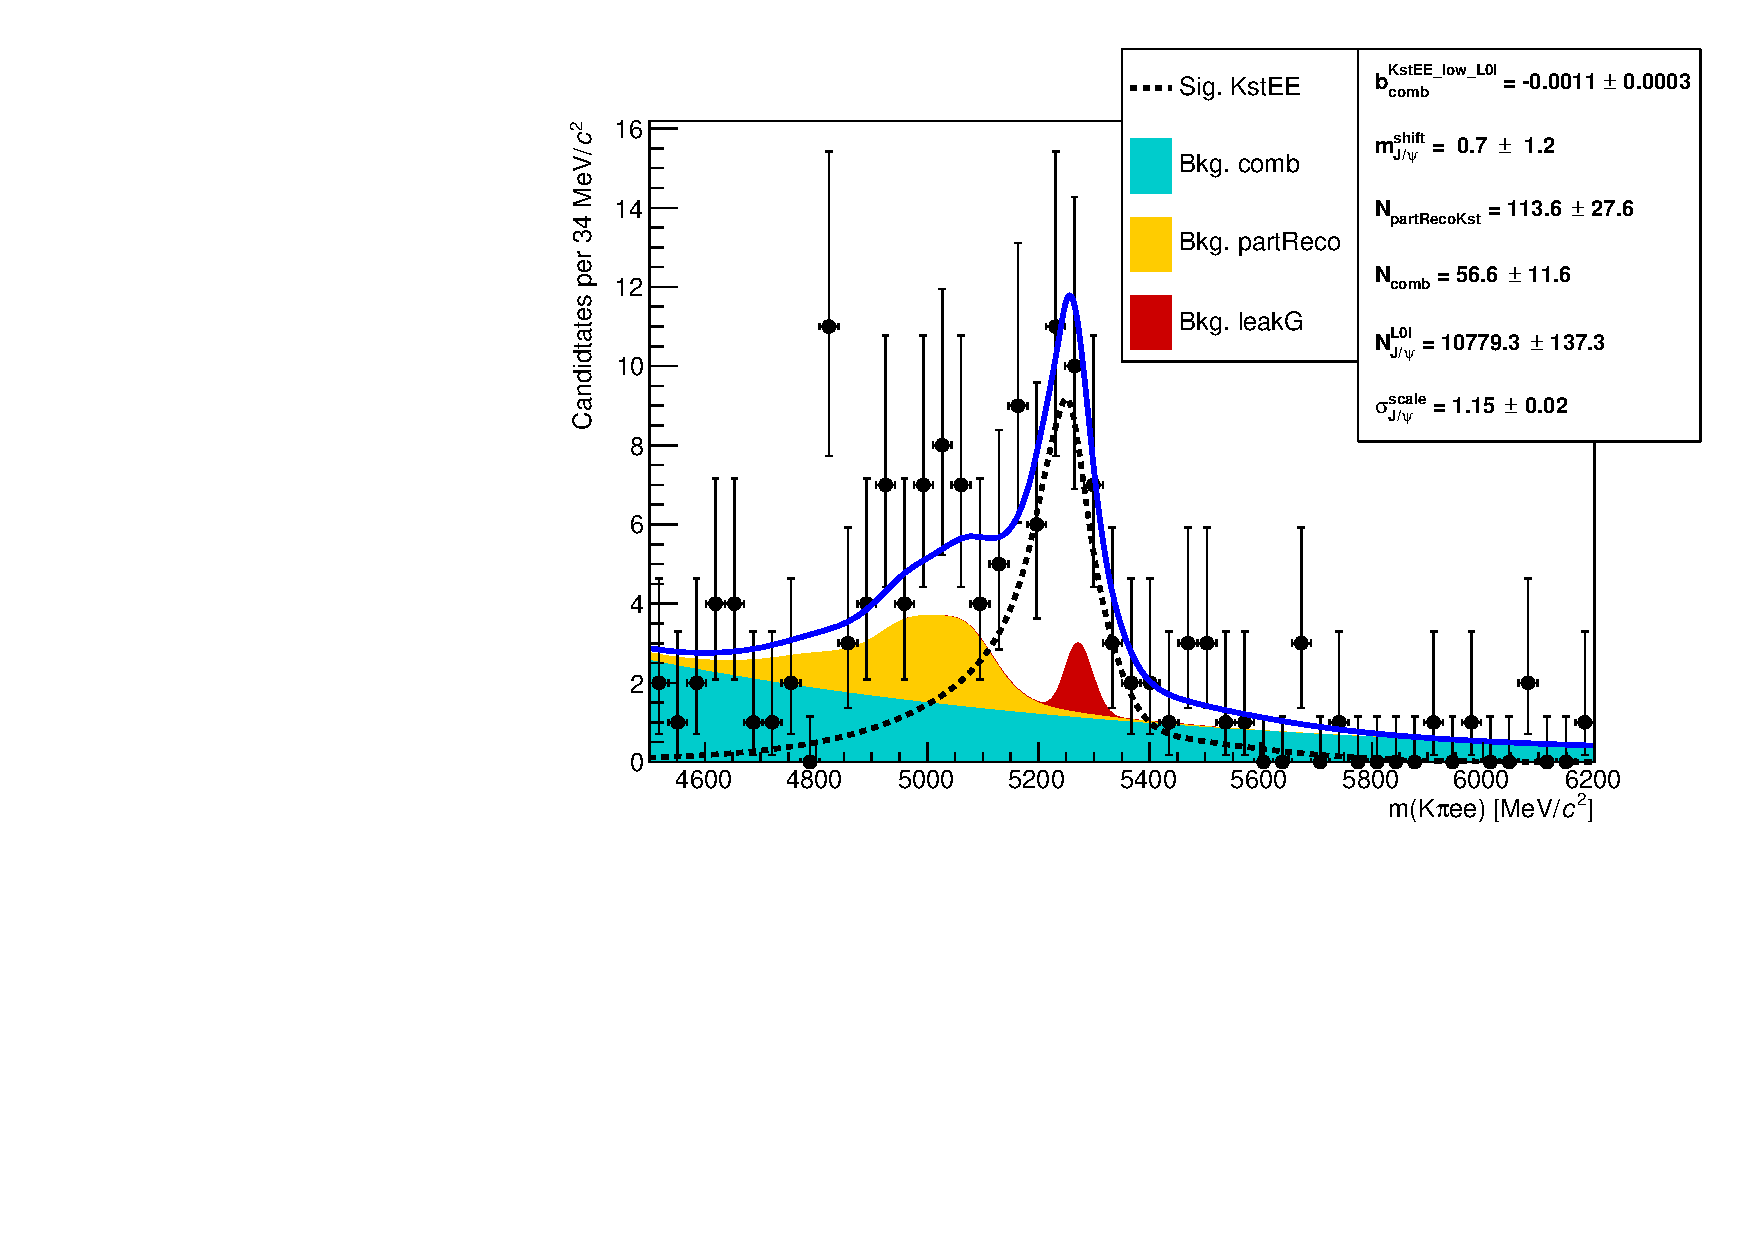
\includegraphics[width=0.49\textwidth]{RKst/figs/Fit/fit_EE/KstEE_low_L0I.pdf}
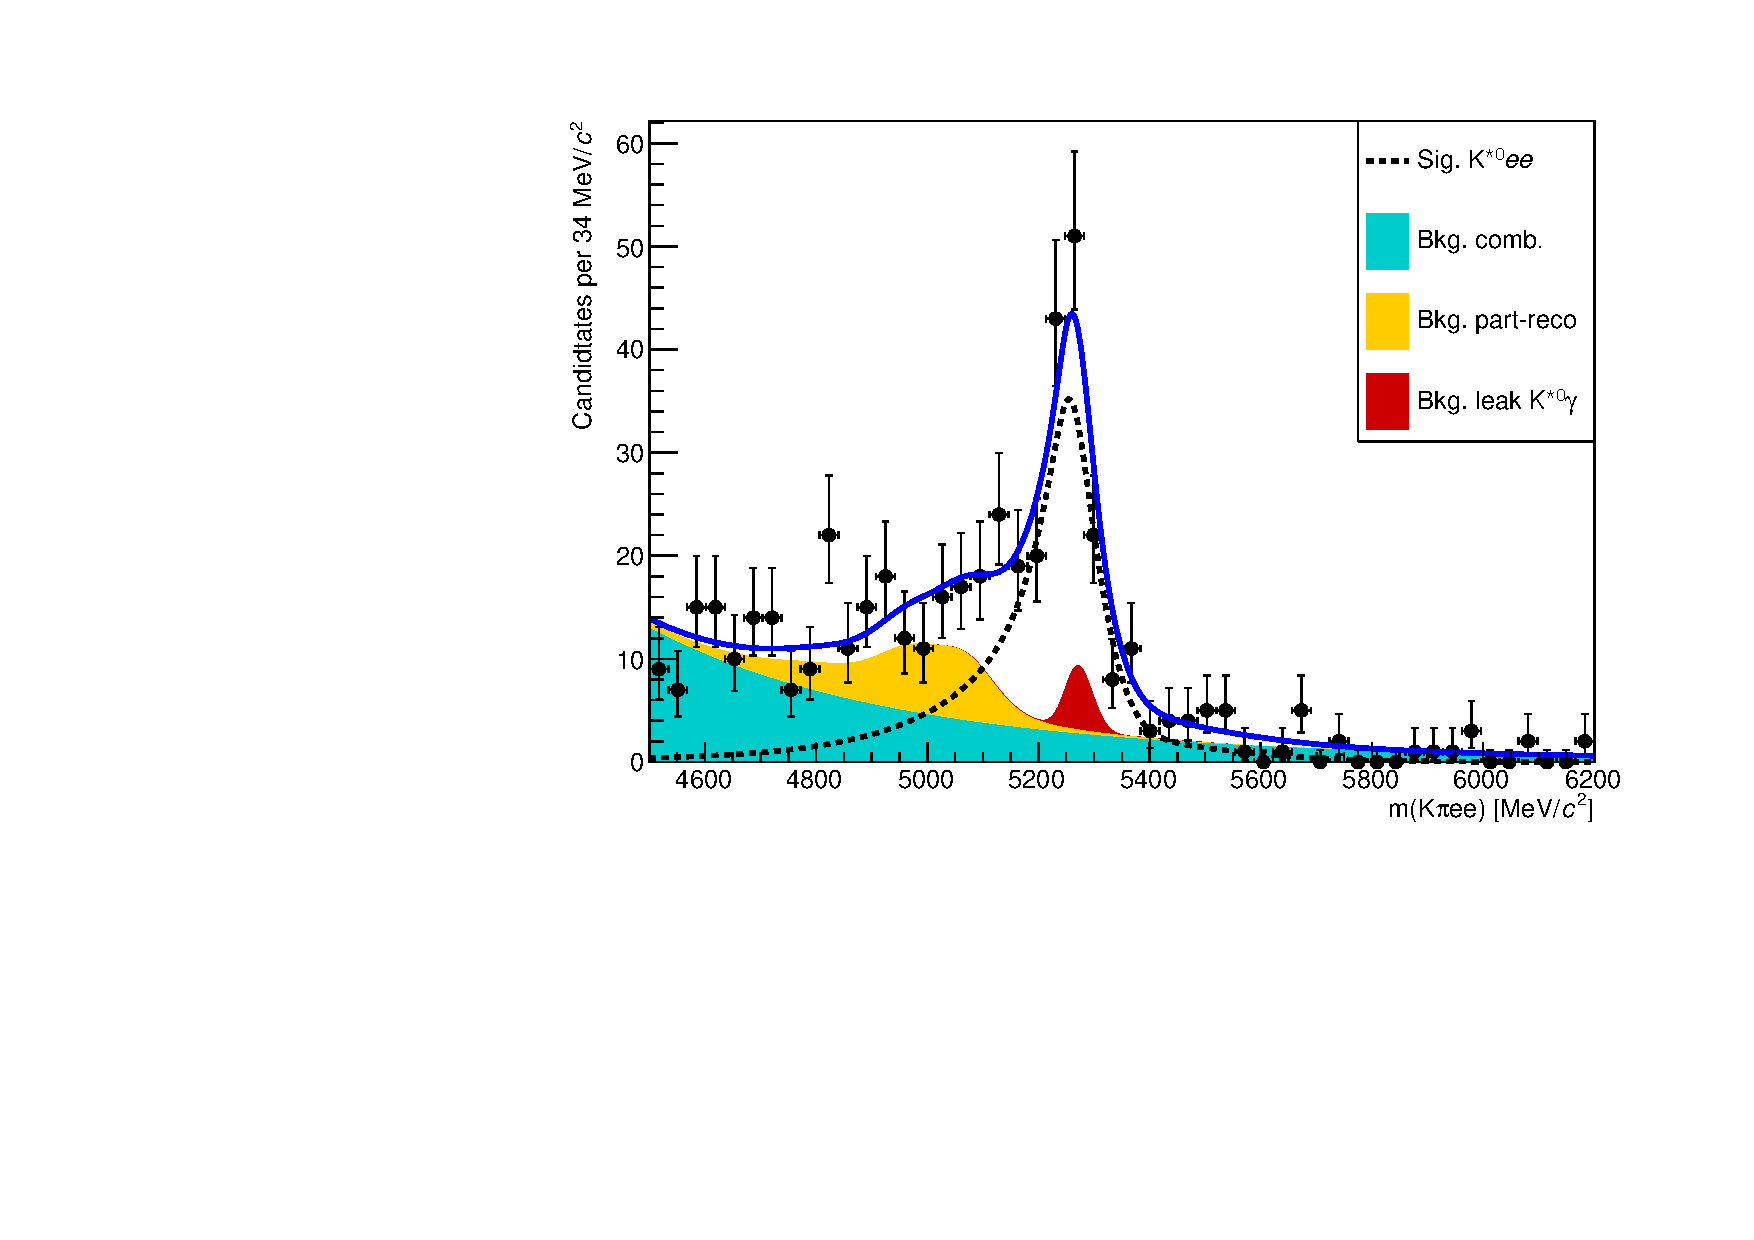
\includegraphics[width=0.49\textwidth]{RKst/figs/Fit/fit_EE/fit_EEl.pdf}
\caption{Fit to the \mKpiee invariant mass of \BdToKstee candidates at low-\qsq in the three trigger categories (L0E, L0H and L0I) separately, and (bottom right) combined. The dashed black line (shaded shapes) represents the signal (background) PDF.}
\label{fig:fitEE_central}
\end{figure}
%
\begin{figure}[h!]
\centering
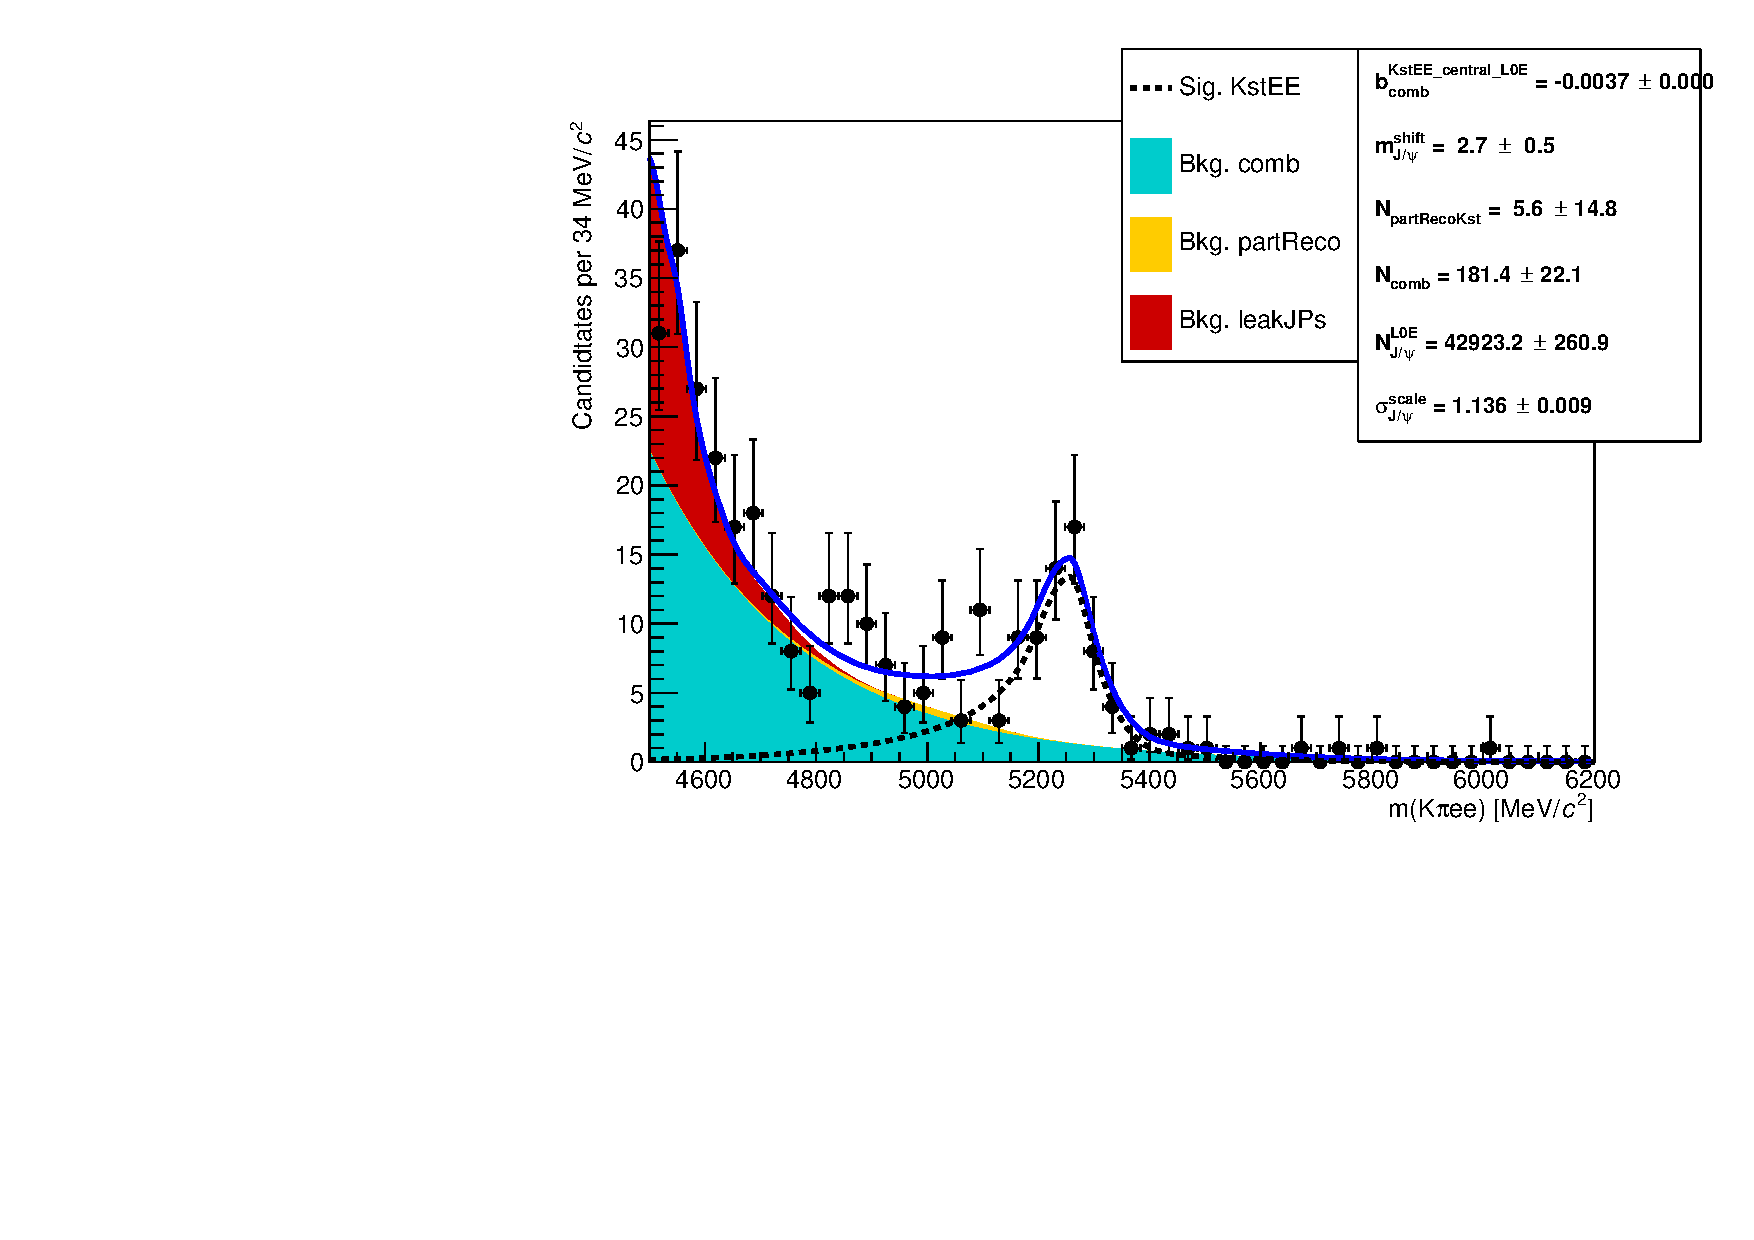
\includegraphics[width=0.49\textwidth]{RKst/figs/Fit/fit_EE/KstEE_central_L0E.pdf}
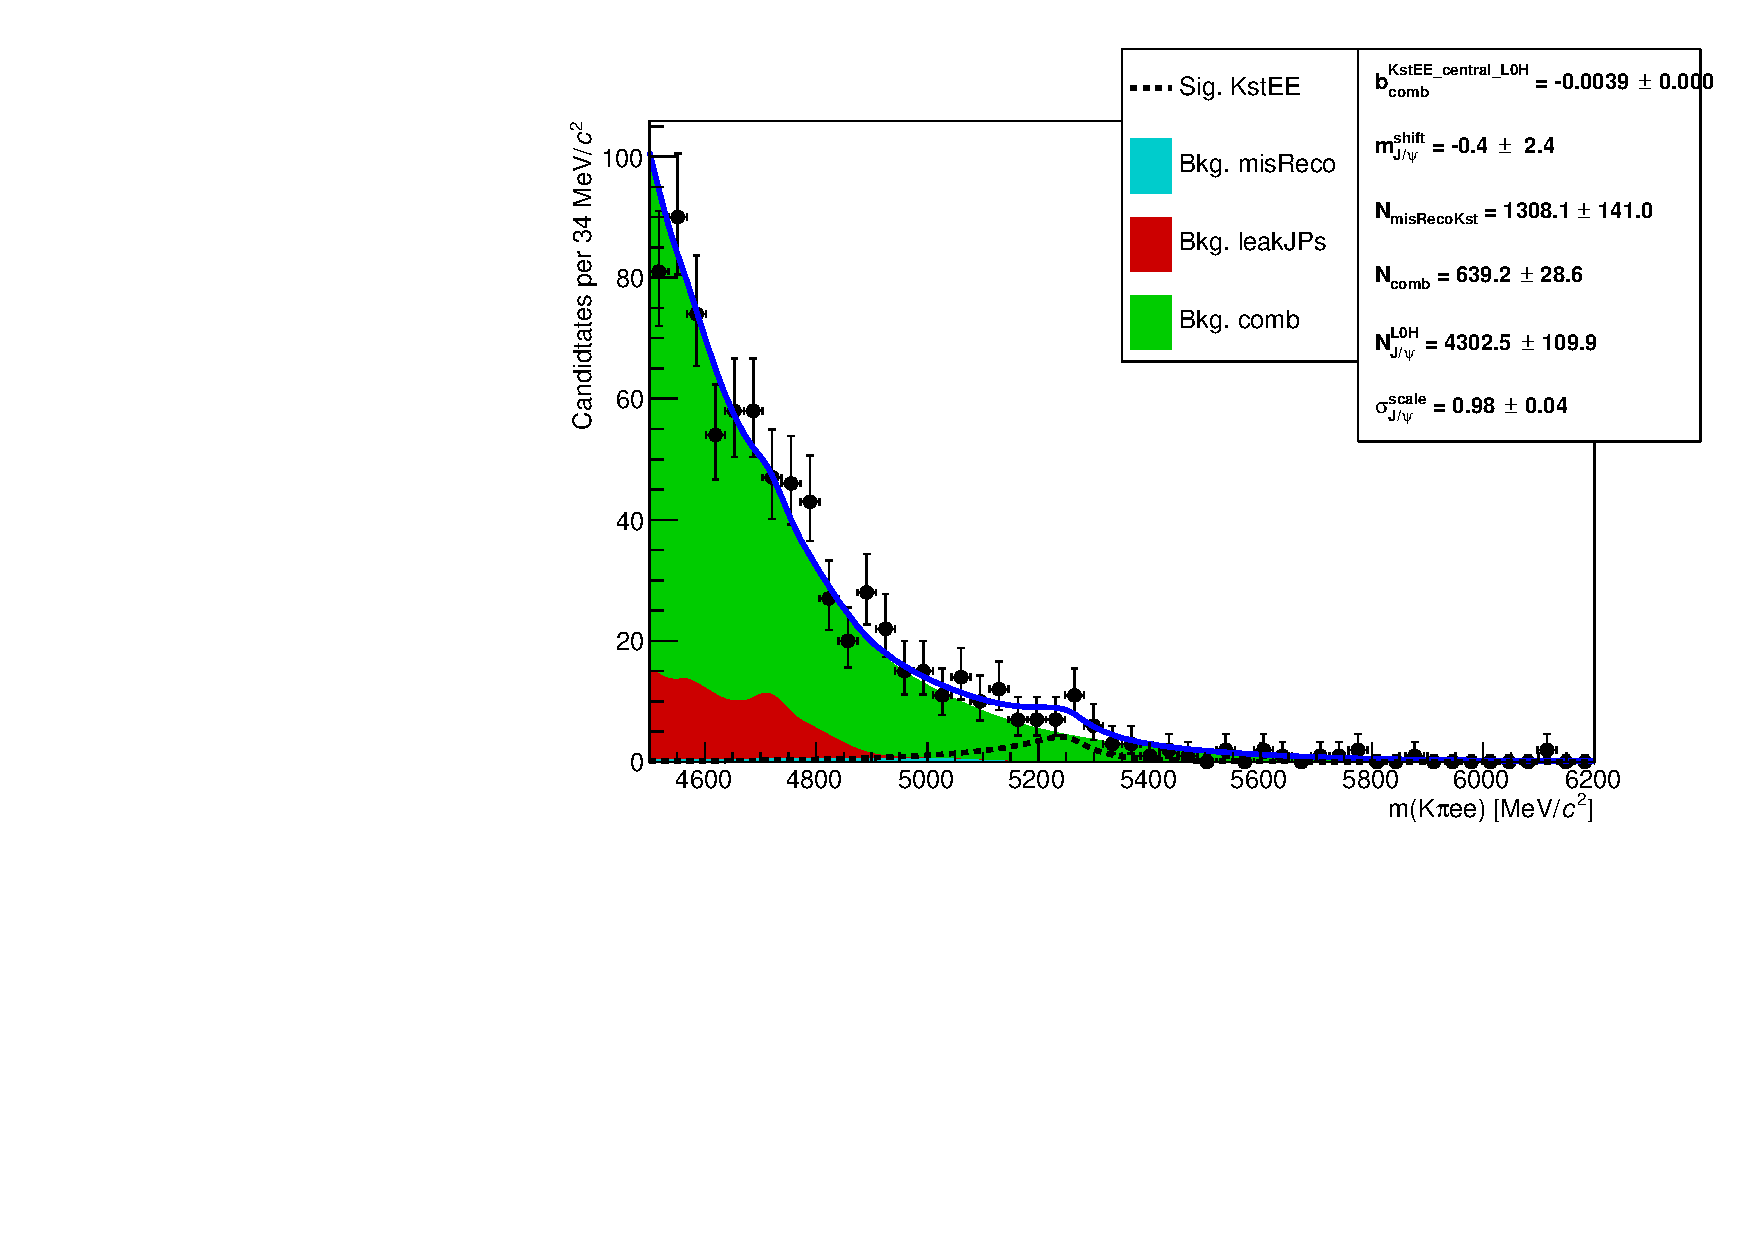
\includegraphics[width=0.49\textwidth]{RKst/figs/Fit/fit_EE/KstEE_central_L0H.pdf}
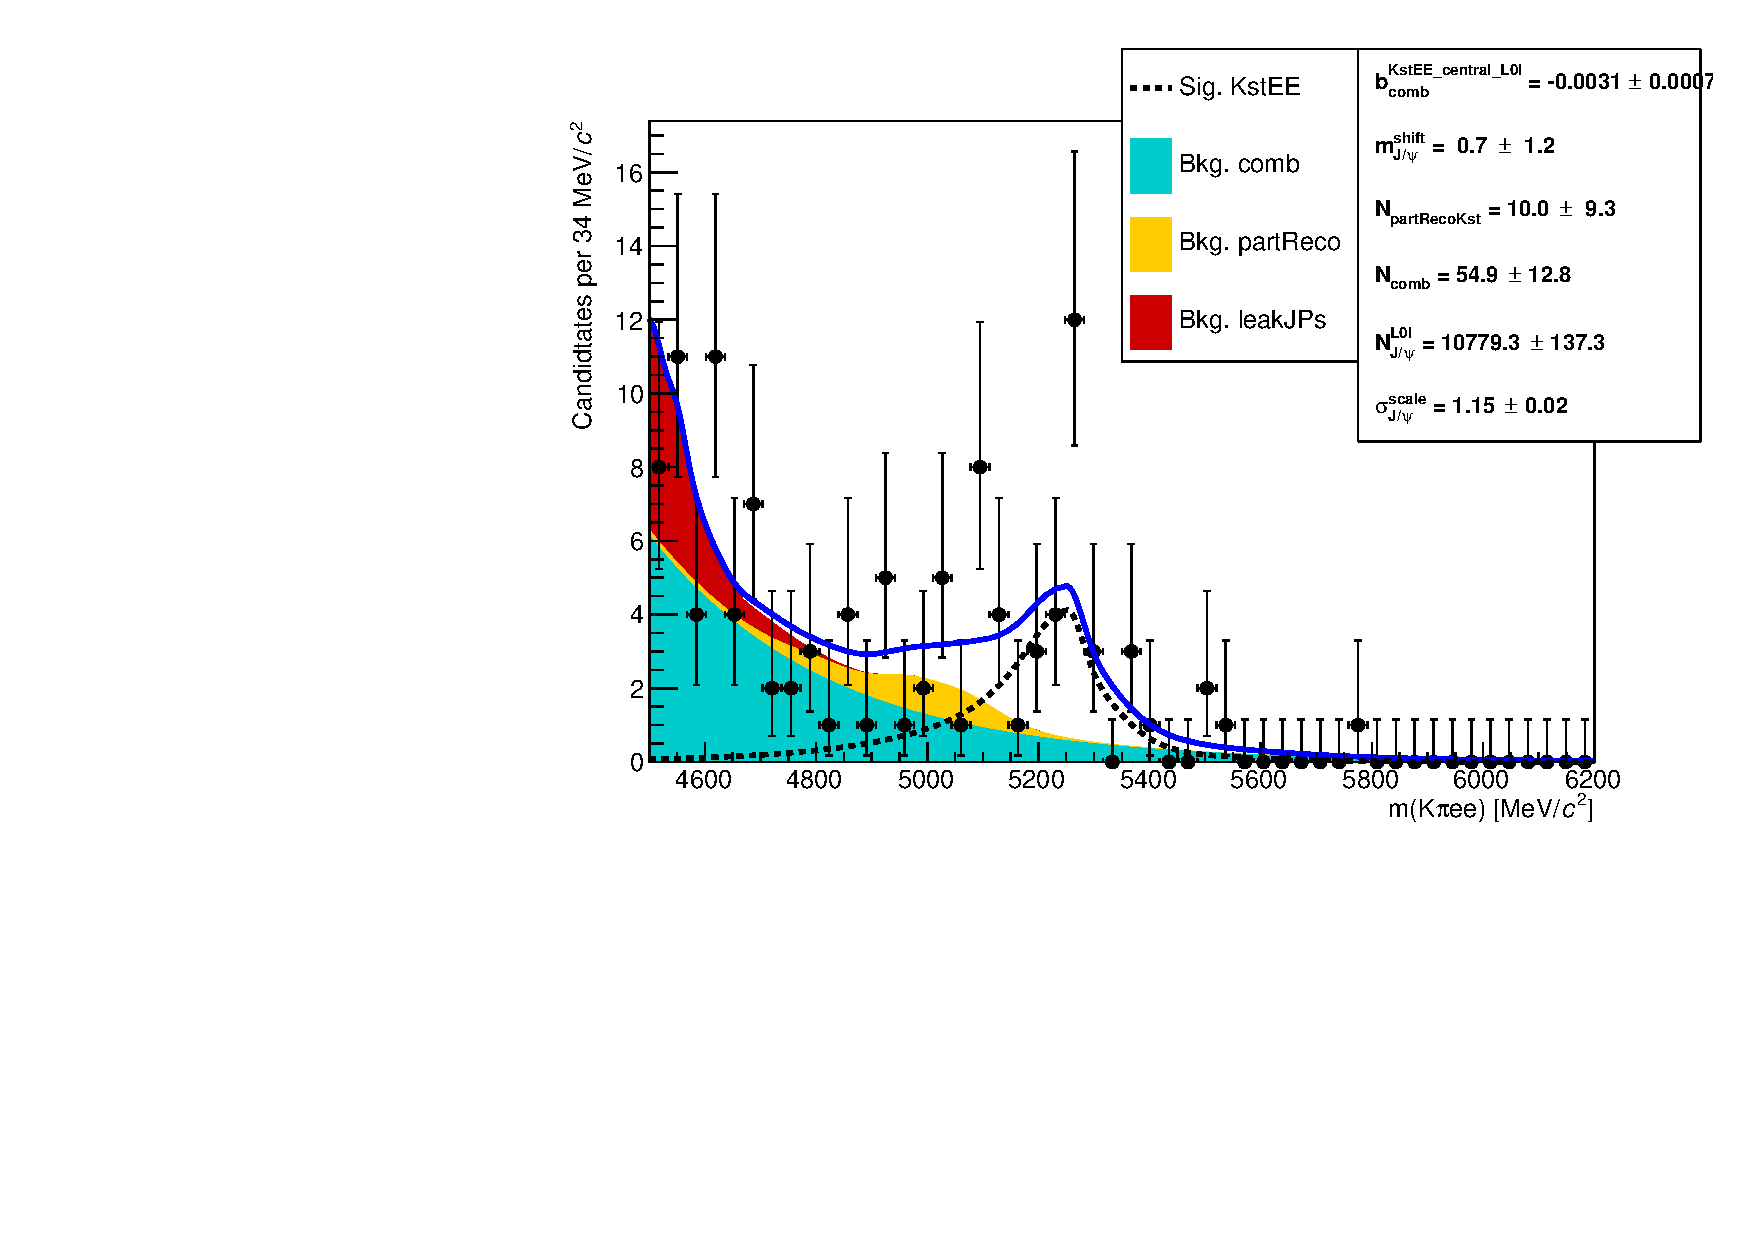
\includegraphics[width=0.49\textwidth]{RKst/figs/Fit/fit_EE/KstEE_central_L0I.pdf}
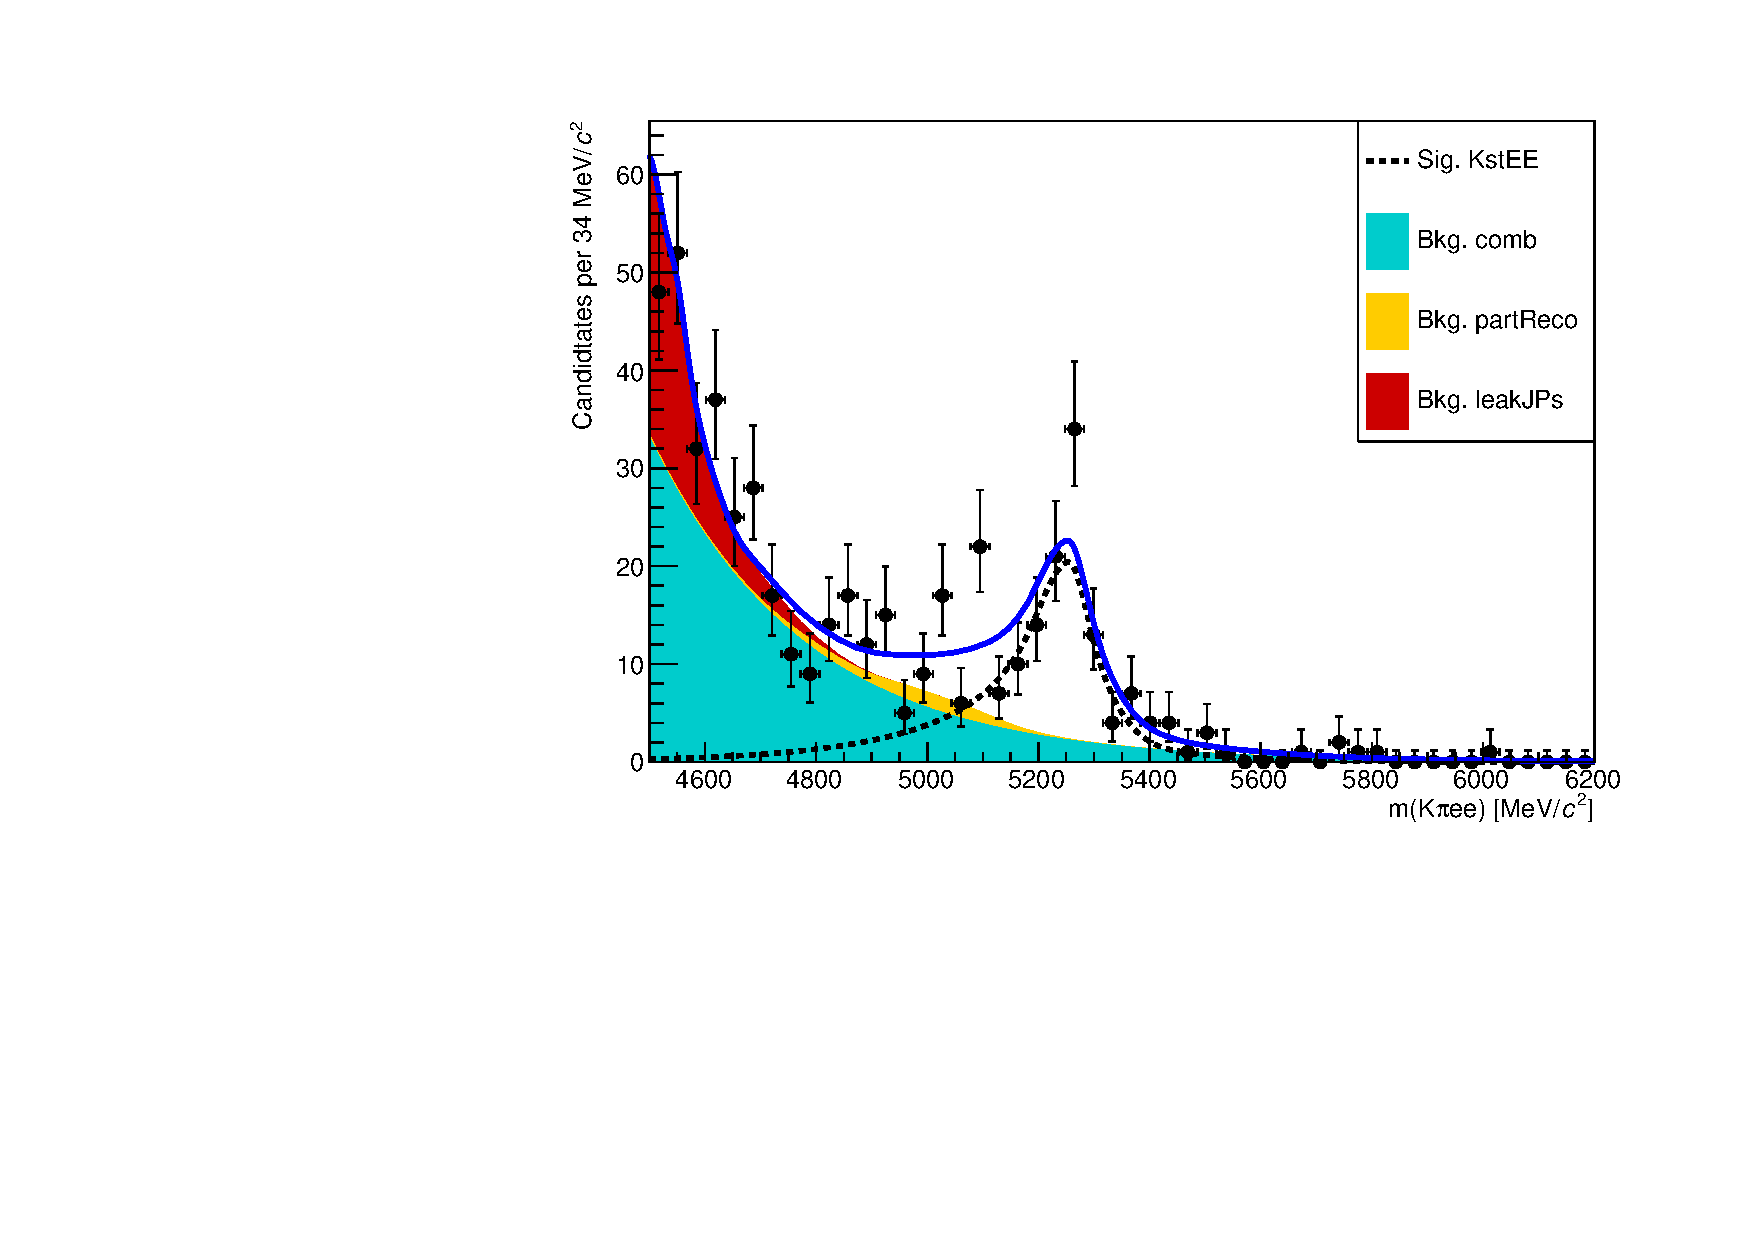
\includegraphics[width=0.49\textwidth]{RKst/figs/Fit/fit_EE/fit_EEc.pdf}
\caption{Fit to the \mKpiee invariant mass of \BdToKstee candidates at central-\qsq in the three trigger categories (L0E, L0H and L0I) separately, and (bottom right) combined. The dashed black line (shaded shapes) represents the signal (background) PDF.}
\label{fig:fitEE_central}
\end{figure}
%
\begin{figure}[h!]
\centering
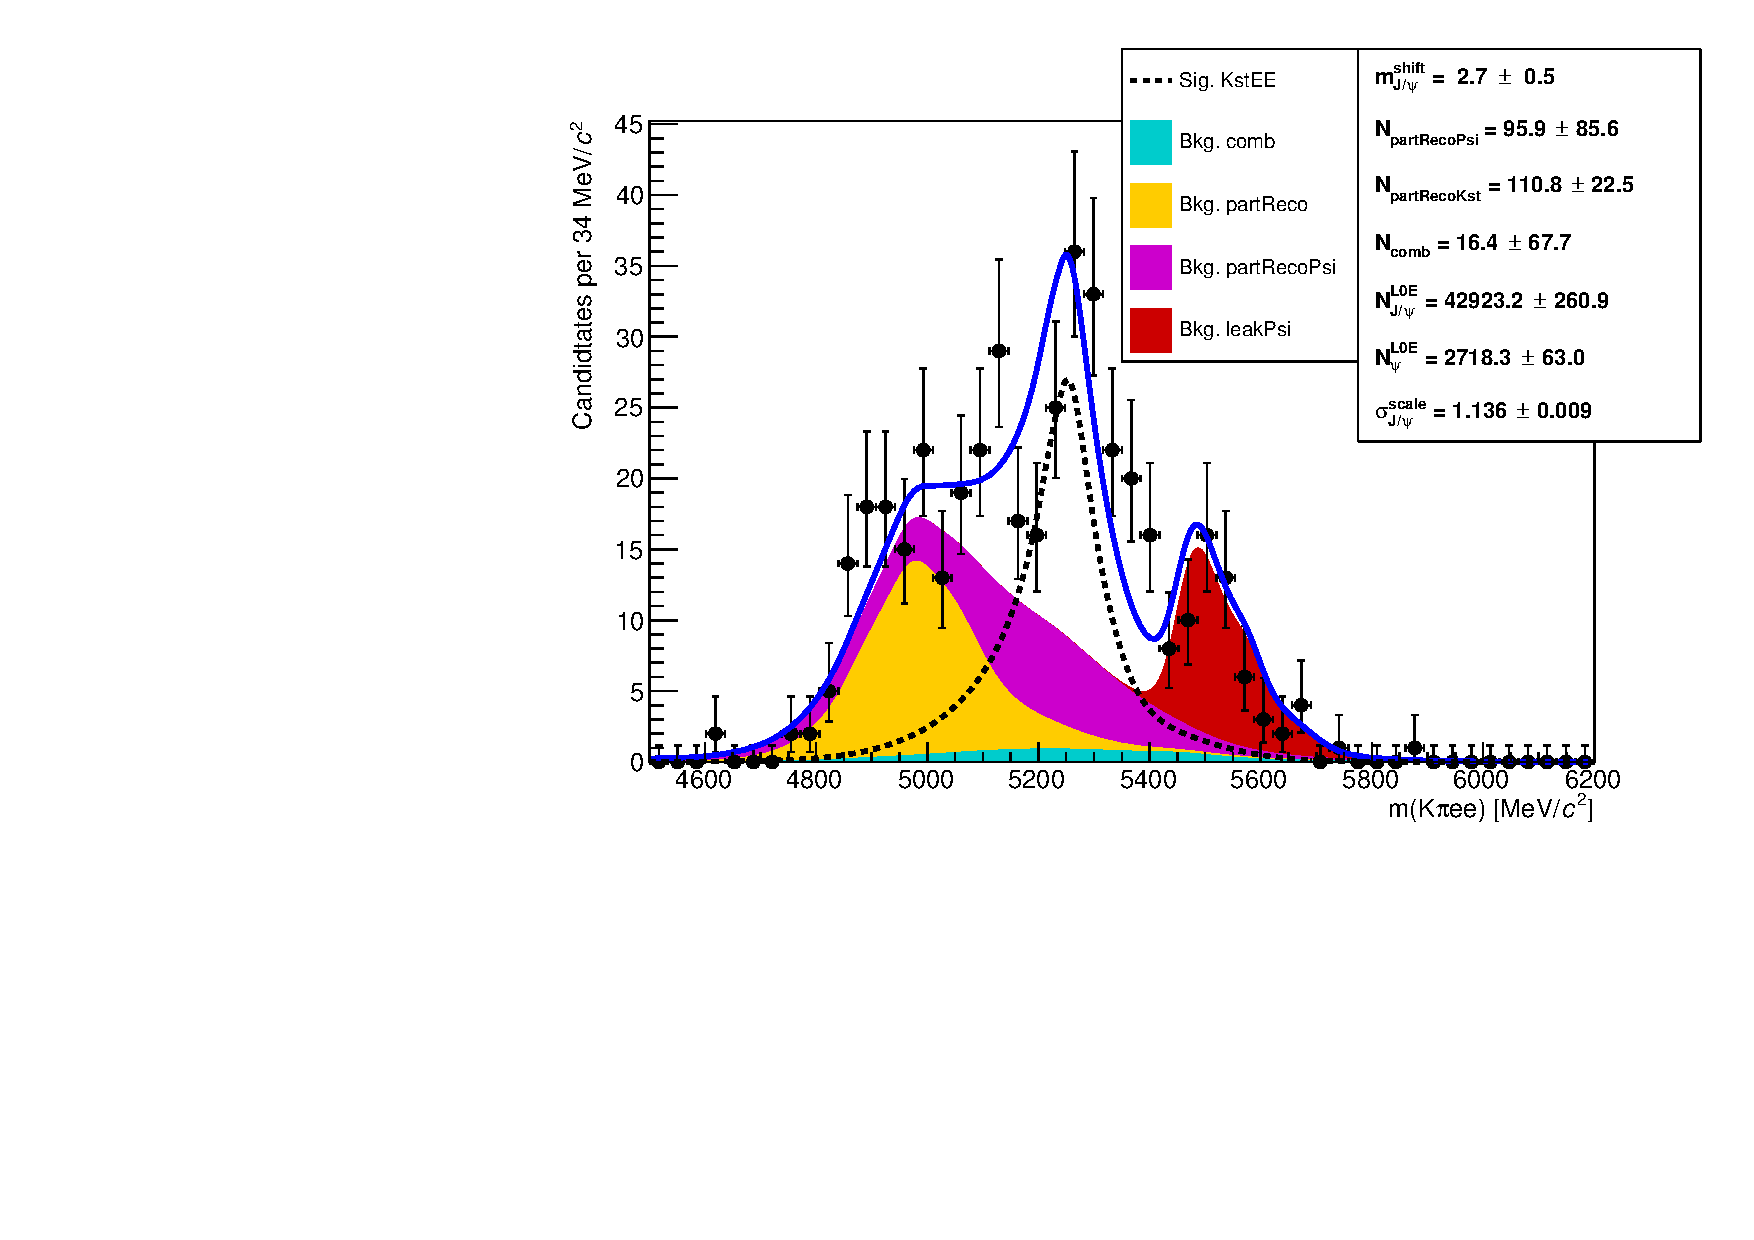
\includegraphics[width=0.49\textwidth]{RKst/figs/Fit/fit_EE/KstEE_high_L0E.pdf}
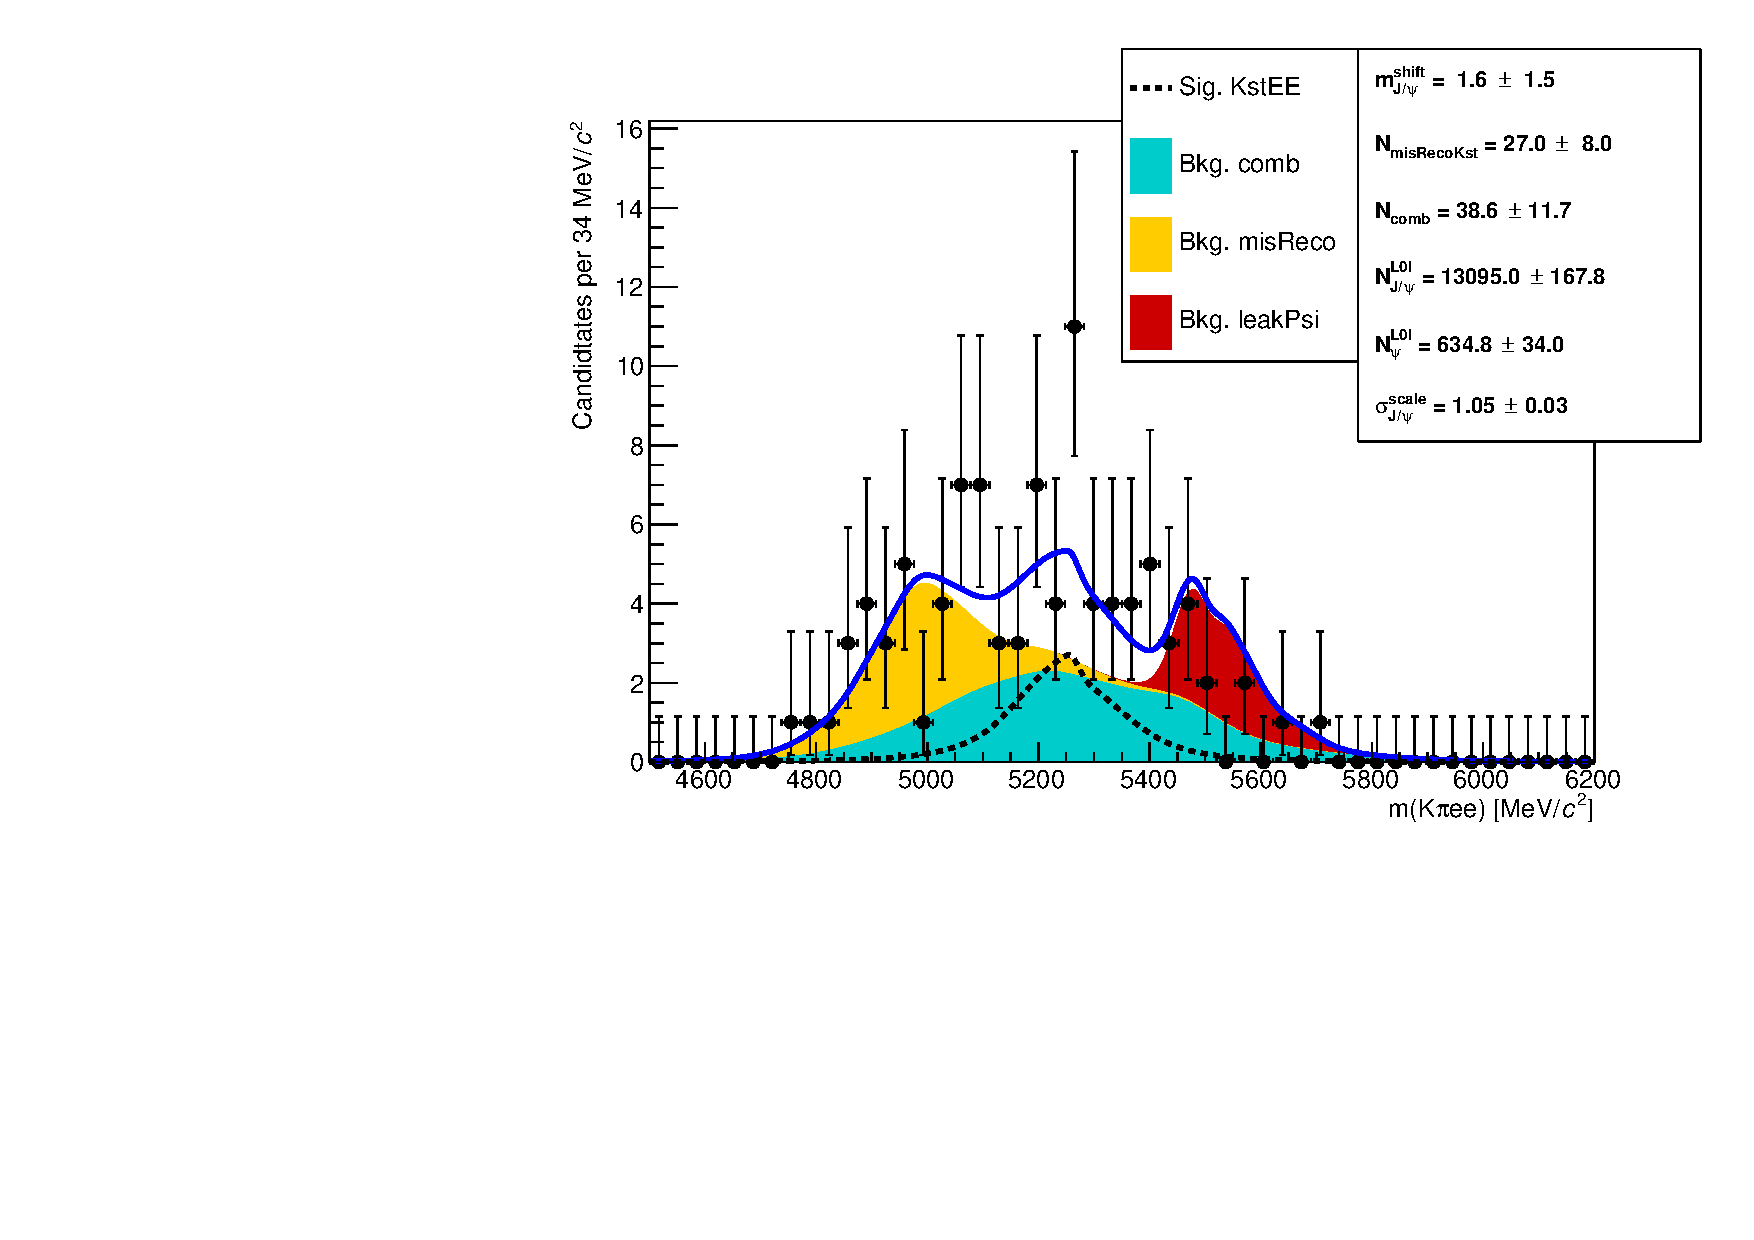
\includegraphics[width=0.49\textwidth]{RKst/figs/Fit/fit_EE/KstEE_high_L0I.pdf}
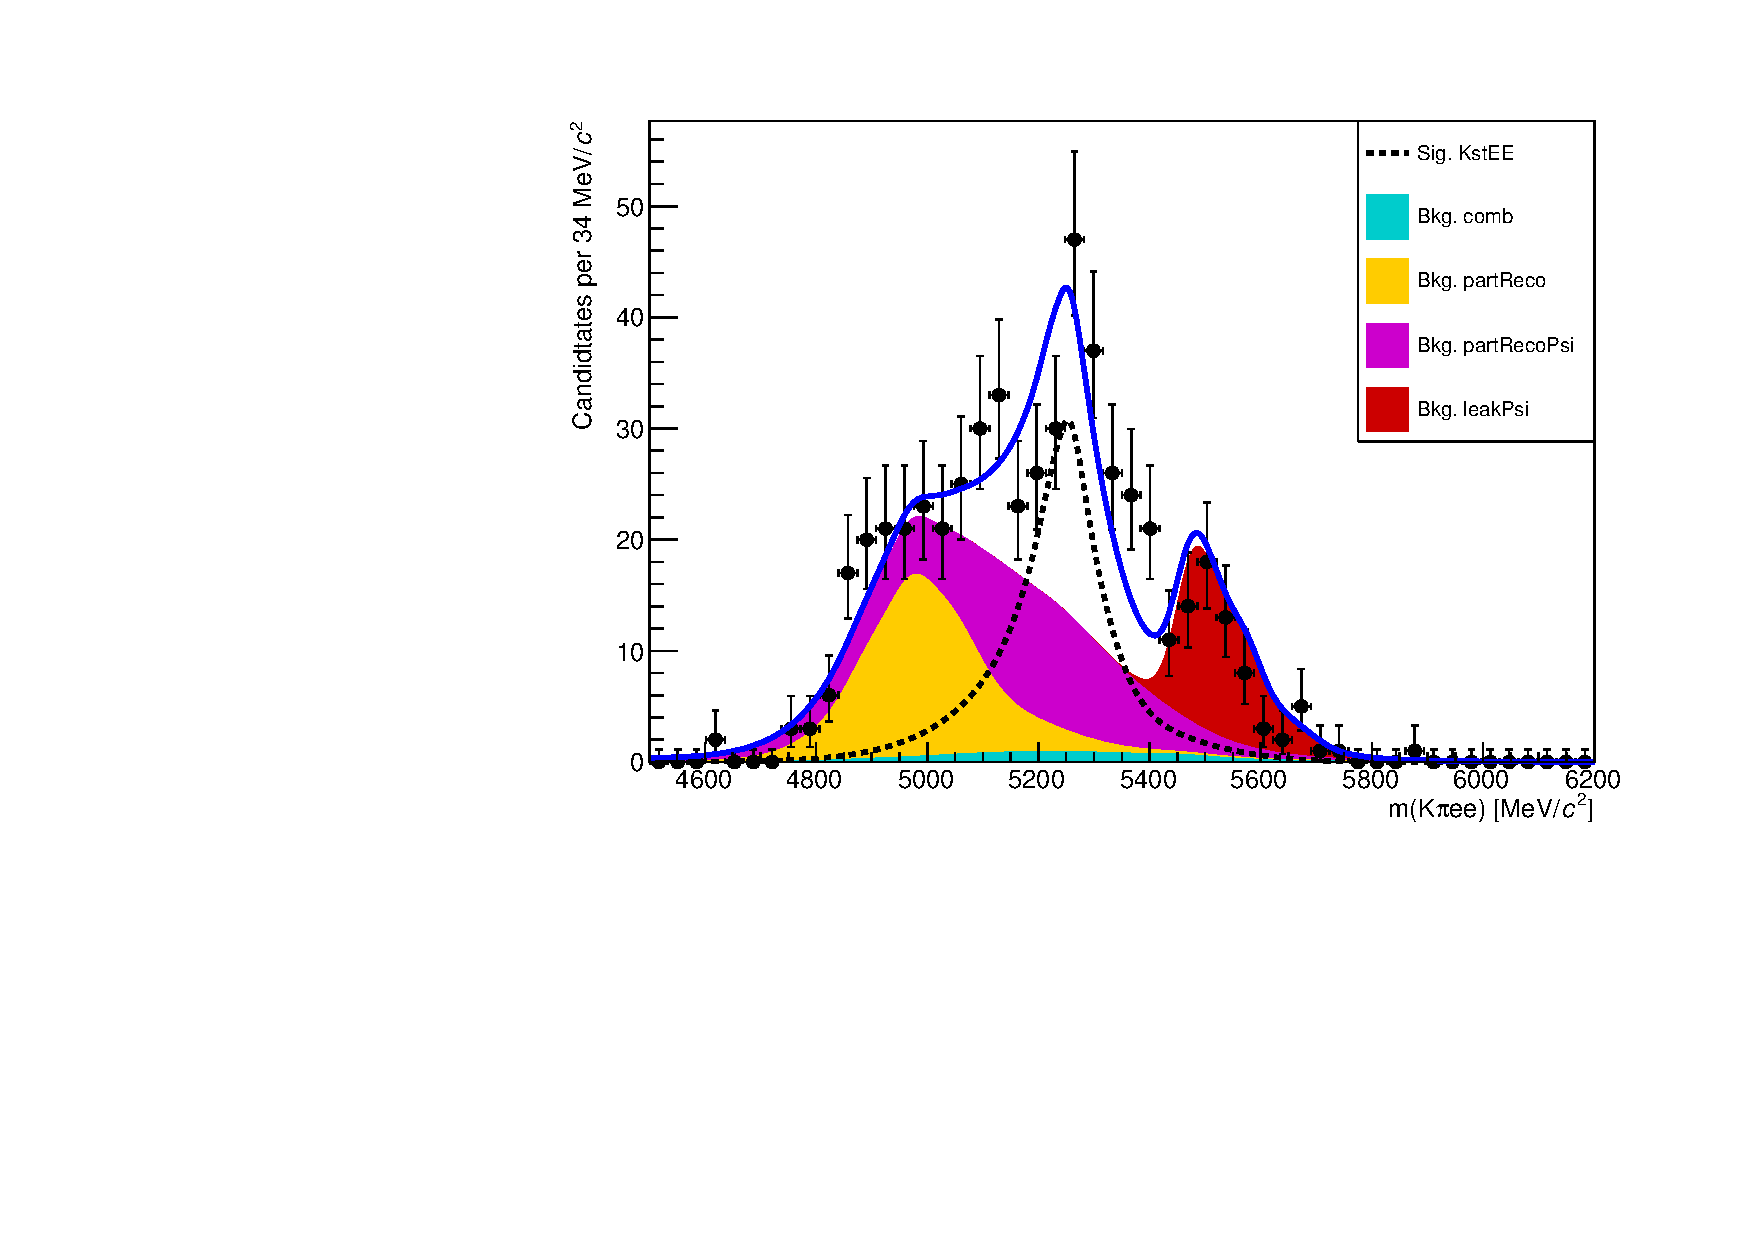
\includegraphics[width=0.49\textwidth]{RKst/figs/Fit/fit_EE/fit_EEh.pdf}
\caption{Fit to the \mKpiee invariant mass of \BdToKstee candidates at high-\qsq in the L0E and L0I trigger categories (top) separately, and (bottom) combined. The dashed black line (shaded shapes) represents the signal (background) PDF.}
\label{fig:fitEE_high}
\end{figure}
